\documentclass[10pt]{article}
\usepackage[utf8]{inputenc}
\usepackage[T1]{fontenc}

\usepackage{amsmath,amssymb,amsfonts,amsthm}
\usepackage[margin=1in, left=1.25in, right=1.25in, top=1in, bottom=1in]{geometry}
\usepackage{booktabs}

\newtheorem{definition}{Definition}
\newtheorem{proposition}{Proposition}
\newtheorem{remark}{Remark}

\usepackage{graphicx}
\usepackage{algorithm}
\usepackage{algorithmic}
\usepackage[linktoc=all, bookmarksdepth=3, pdfstartview=FitH]{hyperref}
\hypersetup{colorlinks=true, linkcolor=blue, filecolor=magenta, urlcolor=cyan}
\urlstyle{same}
\usepackage{multirow}
\usepackage[table,dvipsnames]{xcolor}
\usepackage{subcaption}
\usepackage{caption}
\captionsetup[figure]{name=Fig., labelsep=period}
\usepackage{enumitem}
\usepackage[numbers]{natbib}
\usepackage{cleveref}

\makeatletter
\renewcommand\paragraph{\@startsection{paragraph}{4}{\z@}%
  {1.0ex plus .2ex minus .1ex}{0.4ex}%
  {\normalfont\normalsize}}
\makeatother
\renewcommand{\algorithmicrequire}{\textup{Require:}}
\renewcommand{\algorithmicensure}{\textup{Ensure:}}
\renewcommand{\algorithmicif}{\textup{if}}
\renewcommand{\algorithmicthen}{\textup{then}}
\renewcommand{\algorithmicelse}{\textup{else}}
\renewcommand{\algorithmicelsif}{\textup{else if}}
\renewcommand{\algorithmicendif}{\textup{end if}}
\renewcommand{\algorithmicfor}{\textup{for}}
\renewcommand{\algorithmicforall}{\textup{for all}}
\renewcommand{\algorithmicdo}{\textup{do}}
\renewcommand{\algorithmicendfor}{\textup{end for}}
\renewcommand{\algorithmicwhile}{\textup{while}}
\renewcommand{\algorithmicendwhile}{\textup{end while}}

% Math commands
% math_commands.tex — shared notation for TransitDuet paper
\newcommand{\R}{\mathbb{R}}
\newcommand{\E}{\mathbb{E}}
\newcommand{\N}{\mathbb{N}}
\DeclareMathOperator*{\argmin}{arg\,min}
\DeclareMathOperator*{\argmax}{arg\,max}

% Policies
\newcommand{\piU}{\pi_{\mathrm{U}}}   % upper policy
\newcommand{\piL}{\pi_{\mathrm{L}}}   % lower policy

% State/action spaces
\newcommand{\sU}{s_{\mathrm{U}}}      % upper state
\newcommand{\sL}{s_{\mathrm{L}}}      % lower state
\newcommand{\aU}{a_{\mathrm{U}}}      % upper action
\newcommand{\aL}{a_{\mathrm{L}}}      % lower action

% Advantages
\newcommand{\AU}{A_{\mathrm{U}}}      % upper advantage
\newcommand{\AL}{A_{\mathrm{L}}}      % lower advantage
\newcommand{\AUaug}{\tilde{A}_{\mathrm{U}}}  % augmented upper advantage
\newcommand{\ALaug}{\tilde{A}_{\mathrm{L}}}  % augmented lower advantage

% Target headway
\newcommand{\htarget}{h^{\mathrm{target}}}
\newcommand{\Hpeak}{H_{\mathrm{peak}}}
\newcommand{\Hoff}{H_{\mathrm{off}}}
\newcommand{\Htrans}{H_{\mathrm{trans}}}

% Measurement / constraint
\newcommand{\zvec}{\mathbf{z}}        % measurement vector
\newcommand{\thetavec}{\boldsymbol{\theta}} % OGD weight vector
\newcommand{\Nfleet}{N_{\mathrm{fleet}}}

% Replay buffer, cost
\newcommand{\D}{\mathcal{D}}          % replay buffer
\newcommand{\climit}{c_{\mathrm{lim}}}

% Beta schedule
\newcommand{\betamax}{\beta_{\max}}


% Placeholder command for TBD results
\newcommand{\tbd}[1][]{\textcolor{red}{[TBD#1]}}

\title{TransitDuet: bi-level reinforcement learning for joint bus target-headway planning and holding control}

% \author{Anonymous Authors}
\author{}
\date{}

\begin{document}
\maketitle

\begin{abstract}
We present TransitDuet, a bi-level reinforcement learning framework that jointly optimizes bus timetable planning and real-time holding control.
This joint problem is fundamentally harder than either task in isolation: the planning and control layers operate on different timescales, observe different state spaces, and interact through delayed, asynchronous feedback---properties that violate the synchronous co-execution assumption underlying existing hierarchical reinforcement learning methods.
TransitDuet addresses this through three mechanisms.
First, a goal-conditioned cross-level coupling in the spirit of HIRO: the upper outputs a per-dispatch target-headway shift, and the lower's Lagrangian cost is computed against the resulting goal headway, with no upper-advantage injection into the lower's transitions. This avoids the covariate shift that destabilises a literal cross-advantage augmentation while keeping the upper--lower interaction unidirectional and stable.
Second, a measurement-projection scheme based on online gradient descent enforces fleet-size constraints without reward shaping.
Third, Lagrangian relaxation within the lower policy penalizes headway deviations, converting a hard service-regularity requirement into a soft dual objective.
We evaluate TransitDuet in a calibrated microsimulation of a high-frequency bus corridor with stochastic demand and traffic.
A complementary technique, target-policy-corrected lower SAC (TPC), uses importance-reweighting to align the lower's training distribution with its eventual deployment distribution; combined with the goal-conditioned coupling and trained for 300 episodes per seed, TransitDuet attains the best mean on every metric we report. Across three random seeds and an elastic fleet budget sampled per episode from $[8, 16]$, TransitDuet reduces composite cost by $6.5\%$ ($1.444$ vs $1.544$) and overshoot by $10.4\%$ relative to the strongest hand-tuned fixed timetable, while still improving wait, CV, and overshoot over GA and CMA-ES under the same 300-episode training and held-out evaluation protocol. Seed variance on composite cost is $1.7$--$2.5\times$ smaller than the search baselines, and the learned policy produces a Pareto frontier across nine fleet sizes from a single training run. Generalisation degrades gracefully: wait rises only $25\%$ when route variance is doubled beyond the training distribution.
\end{abstract}


\noindent Keywords: bus holding control; target-headway planning; hierarchical reinforcement learning; multi-timescale control; constrained optimization.

\section{Introduction}
\label{sec:intro}

High-frequency bus systems face a persistent coordination failure.
Timetables are planned offline to balance fleet utilization against passenger demand, yet the headways they prescribe degrade within minutes once buses encounter stochastic traffic and boarding delays.
Real-time holding control can restore regularity, but only within the headway structure it inherits.
When the timetable itself is poorly matched to demand---dispatching too few buses in the peak or too many in the off-peak---no amount of holding can recover acceptable service.
Planning and control are thus coupled: the quality of one layer bounds the achievable performance of the other.

Despite this coupling, existing work treats the two problems separately.
The timetable optimization literature formulates headway or frequency design as mixed-integer programs solved offline \citep{gkiotsalitis2021bus}, while the holding control literature trains reinforcement learning (RL) agents that take the timetable as given \citep{wang2020real}.
Joint optimization would seem a natural application of hierarchical RL, yet three gaps prevent a straightforward application.

\paragraph{Asynchrony between planning and control.}
Hierarchical RL frameworks such as the options framework \citep{sutton1999between} and goal-conditioned methods like HIRO \citep{nachum2018data} assume that the upper and lower levels share a common state clock or that the upper level sets subgoals consumed by the lower level within a fixed horizon.
In bus operations, the upper policy acts at dispatch events (once per bus departure), while the lower policy acts at every station arrival across all active buses.
The two levels observe different state spaces---the upper level sees route-level demand forecasts and fleet status, whereas the lower level sees per-bus headway deviations and passenger loads---and interact through delayed feedback spanning an entire trip lifecycle.
No shared clock or fixed subgoal horizon exists.

\paragraph{Cross-advantage under asynchrony.}
\citet{pan2024roboduet} recently introduced cross-advantage augmentation for bi-level robot locomotion, where an upper style policy and a lower tracking policy execute synchronously on the same state.
Their augmented advantage $\AUaug = \AU + \beta \AL$ directly sums the two advantages at each time step.
This elegant mechanism breaks down when the two levels operate on different timescales with different state and action spaces: there is no single time step at which $\AU$ and $\AL$ are jointly defined.
Generalising cross-level coupling to the asynchronous, multi-timescale setting requires propagating execution outcomes (rather than per-step advantages) over the variable-length trip lifecycle initiated by each dispatch, and exposing lower-level holding statistics to the upper policy through state augmentation rather than reward backflow.

\paragraph{Fleet and regularity constraints.}
Bus operations impose feasibility-style constraints---a fleet-size budget $\Nfleet$ and bounded headway deviation---that naive reward shaping handles poorly.
Constrained RL methods such as RCPO \citep{tessler2019reward} address single-level constraint satisfaction but do not account for constraints that span a bi-level structure, where the upper level controls resource allocation and the lower level controls service regularity.

\medskip

We propose TransitDuet, a bi-level RL framework that addresses all three gaps.
The upper policy $\piU$ outputs a per-dispatch target-headway shift $\delta_t \in [-120, 120]$\,s at each dispatch event; the lower's headway target for that trip is reset to $\htarget + \delta_t$. The lower policy $\piL$, a soft actor-critic with Lagrangian penalties \citep{haarnoja2018soft}, selects holding times at every station arrival with parameter sharing across buses, and its constraint is computed against the dispatch-specific goal headway.
This goal-conditioned coupling, in the spirit of HIRO~\citep{nachum2018data}, replaces the literal cross-advantage augmentation of RoboDuet~\citep{pan2024roboduet} (Section~\ref{sec:tap}); two auxiliary upper-only signals (a holding-feedback state channel and a per-dispatch hindsight credit on the upper reward) provide credit assignment without injecting upper signals into the lower's transitions.
Lower-policy training begins with a $30$-episode warmup during which the upper is held at $\delta_t = 0$, after which the goal channel engages.
Fleet-size feasibility is enforced by a $\thetavec$-weighted online gradient descent projection on the measurement vector $\zvec$ of dispatched buses, inspired by the ApproPO framework \citep{miryoosefi2019reinforcement}, while headway uniformity enters the lower-level objective through Lagrangian relaxation.

\paragraph{Contributions.}
The specific contributions of this paper are:
\begin{enumerate}
    \item \textbf{Goal-conditioned cross-level coupling.} We adopt a HIRO-style goal-conditioned coupling~\citep{nachum2018data}: the upper outputs a per-dispatch target-headway shift, and the lower's Lagrangian cost is computed against the resulting goal headway, with no upper-advantage injection into the lower's transitions. We compare this end-to-end against (i) a literal cross-advantage augmentation following HAAR~\citep{li2019hierarchical} with a PIPER-style reachability gate~\citep{singh2024piper}, and (ii) a three-channel coupling that uses $\delta_t$ as a launch-time perturbation with hindsight reward credit; the goal-conditioned design has the best mean composite cost ($1.444$ vs $1.499$ vs $1.492$) and the lowest seed variance ($1.7$--$2.0\times$ tighter than the alternatives) on the same evaluation protocol.
    \item \textbf{Joint timetable--holding formulation.} We cast bus timetable planning and holding control as a bi-level Markov decision process with heterogeneous state-action spaces and asynchronous transitions, providing a formal problem structure absent from prior bus RL work.
    \item \textbf{Constraint satisfaction via $\thetavec$-OGD and Lagrangian relaxation.} We integrate measurement-projection constraints at the upper level and dual-variable penalties at the lower level, handling fleet feasibility and headway regularity without reward shaping.
    \item \textbf{Target-policy-corrected lower SAC (TPC).} We identify a previously overlooked failure mode of joint bi-level RL on tightly coupled control: the lower policy is trained alongside an exploring upper policy, biasing the lower's training distribution away from deployment. We address this via importance-weighted lower SAC against an EMA "deployment" upper policy, with validation-based checkpoint selection.
    \item \textbf{Empirical evaluation on a calibrated corridor.} On a stochastic microsimulation under a unified 300-episode training and held-out evaluation protocol, TransitDuet attains the best mean on every metric we report: composite cost $1.444$ vs $1.504$ for the next-best baseline (CMA-ES, $-4.0\%$) and $1.544$ for Fixed ($-6.5\%$), with seed variance $1.7$--$2.5\times$ smaller than the search baselines.
\end{enumerate}

\paragraph{Results preview.}
We evaluate on a high-frequency bus corridor with 22 stations, 264 daily trips, demand stochasticity $\sigma_{\mathrm{demand}} = 0.15$, and elastic fleet $\Nfleet \in [8, 16]$ sampled per episode. Under a unified 300-episode training and held-out evaluation protocol, TransitDuet attains the best mean on wait, CV, overshoot, and composite cost simultaneously --- improvements of $5.5$/$6.4$/$10.4$/$6.5\%$ respectively over the strongest hand-tuned Fixed timetable --- and the lowest composite-cost variance of any method, while degrading only $25\%$ on wait when route stochasticity is doubled beyond the training distribution.

\paragraph{Paper organization.}
\Cref{sec:related} reviews related work in timetable optimization, bus holding RL, and hierarchical RL.
\Cref{sec:problem} formalizes the bi-level MDP.
\Cref{sec:method} presents the TransitDuet architecture, the cross-level coupling channels, and the constraint-handling mechanisms.
\Cref{sec:experiments} describes the simulation environment and reports results.
\Cref{sec:discussion} discusses limitations and extensions.
\Cref{sec:conclusion} concludes.

\section{Related work}\label{sec:related}
\label{sec:related_work}

\subsection{Reinforcement learning for bus holding control}
\label{subsec:rl_holding}

The application of reinforcement learning to real-time bus holding control has attracted considerable attention in recent years, driven by the promise of adaptive policies that can respond to stochastic passenger demand and traffic conditions. \citet{alesiani2018reinforcement} formulated holding for high-frequency services as a value-based RL problem, showing that a Q-learning controller could reduce headway dispersion compared to schedule-based rules. \citet{wang2020real} subsequently studied multi-agent deep RL for the bus-bunching problem, casting each bus as an independent agent with a shared policy network and demonstrating that learned holding actions stabilize headways across an entire corridor without explicit communication. The shared-parameter paradigm common to these works scales gracefully with fleet size and implicitly encourages cooperative behavior through shared gradient updates.

Despite these advances, existing RL-based holding controllers share a fundamental limitation: they operate under a fixed, externally supplied timetable. The planned departure times and target headways are treated as immutable inputs, meaning that the holding policy has no mechanism to communicate execution-level feedback---such as systematic schedule infeasibility or recurrent bunching patterns---back to the planning stage. When the timetable itself is poorly calibrated to actual operating conditions, even an optimal holding policy can only mitigate, not resolve, the resulting service irregularity. TransitDuet addresses this gap by embedding the holding controller as the low-level agent within a bi-level framework, where real-time execution performance directly shapes the timetable through Temporal Advantage Propagation.

\subsection{Bus timetable optimization}
\label{subsec:timetable_opt}

Timetable design has traditionally been approached through mathematical programming and metaheuristic search. \citet{ibarra2015planning} formulated the problem as a mixed-integer program that jointly determines departure times and vehicle assignments to minimize a weighted combination of passenger waiting time and operator cost, solving it via branch-and-bound with valid inequalities. \citet{gkiotsalitis2021bus} proposed a bi-level model in which the upper level selects headways to minimize total passenger cost while the lower level solves a vehicle scheduling problem, solved using an adaptive large neighborhood search. Frequency-setting variants, such as the work of \citet{cats2019frequency}, optimize the number of departures per period rather than individual departure times, and typically rely on assignment models to estimate passenger flows under each candidate frequency vector.

A common thread in this literature is the reliance on static demand forecasts and deterministic travel-time assumptions. Timetables are optimized offline against expected conditions and then handed off to operations without a feedback loop. When actual conditions deviate---due to traffic incidents, demand surges, or driver variability---the timetable may become infeasible, and holding controllers are left to absorb the mismatch. Moreover, the combinatorial structure of these formulations limits scalability: solution times grow rapidly with the number of trips and stops, making re-optimization during the operating day impractical. TransitDuet replaces this open-loop paradigm with a closed-loop one. The high-level agent learns a timetable policy that maps aggregate state features to departure-time adjustments, and it receives gradient signals from low-level execution via the cross-level coupling channels described in Section~\ref{sec:tap}, enabling the planner to adapt its decisions based on how well the resulting schedule can actually be executed.

\subsection{Hierarchical and multi-timescale reinforcement learning}
\label{subsec:hierarchical_rl}

Hierarchical reinforcement learning decomposes complex tasks into temporally extended sub-problems. The options framework of \citet{sutton1999between} introduced the notion of temporally abstract actions, each consisting of an initiation set, an intra-option policy, and a termination condition, enabling planning over multiple timescales within a single MDP. Feudal networks \citep{vezhnevets2017feudal} operationalize this idea with a manager that sets sub-goals in a learned latent space and a worker that executes primitive actions to reach them, training both levels end-to-end with the manager's policy gradient modulated by the worker's goal-reaching success. HIRO \citep{nachum2018data} further improved sample efficiency by introducing off-policy corrections that relabel high-level goals in hindsight, making hierarchical training practical in continuous-control domains. Beyond goal-conditioned hierarchies, \citet{lee2020reinforcement} and \citet{metelli2020control} studied the multi-timescale setting more broadly, analyzing the interaction between agents operating at different decision frequencies and establishing regret bounds for the resulting non-stationary sub-problems.

While these methods provide powerful abstractions for temporal hierarchy, most assume either synchronous execution---where the high-level decision triggers immediately before a fixed-length sequence of low-level steps---or a shared state space across levels. In transit operations, the planning and control timescales are fundamentally asynchronous: the timetable agent acts once per planning horizon (e.g., every 15--30 minutes), while the holding agent acts at every stop visit (every 1--3 minutes), and the two levels observe different state representations at non-aligned decision epochs. TransitDuet handles this asynchrony through three coupling channels (Section~\ref{sec:tap}): a state channel exposing lower-level holding statistics to the upper policy, an action channel through which the upper offset directly perturbs the lower's environment, and a reward channel that backfills each dispatch's reward with a hindsight credit derived from the realised inter-dispatch gap. We initially attempted a literal asynchronous extension of RoboDuet-style cross-advantage augmentation, but the per-step advantage scales of the upper and lower policies differed substantially across a trip lifecycle and the resulting training was unstable; the reward-channel design described in this paper proved markedly more reliable.

\subsection{Constrained reinforcement learning}
\label{subsec:constrained_rl}

Many practical RL deployments must satisfy constraints beyond reward maximization. Lagrangian relaxation is the most widely used approach: \citet{tessler2019reward} proposed reward-constrained policy optimization, which augments the policy gradient with dual variables corresponding to cost constraints and performs primal-dual updates to steer the policy toward feasibility. \citet{stooke2020responsive} improved upon this with PID-based Lagrange multiplier updates that reduce oscillation and speed convergence in the constrained setting. These methods are effective for soft constraints, where occasional small violations are tolerable, but they offer no worst-case guarantees---the Lagrange multiplier may fail to grow fast enough to prevent persistent violations during training.

For settings that demand hard constraint satisfaction, \citet{miryoosefi2019reinforcement} introduced ApproPO, which formulates the constrained problem as an online convex optimization over the space of occupancy measures and applies a measurement-based projection oracle to enforce feasibility at every iterate. The $\theta$-OGD variant provides a practical implementation that projects policy parameters onto the feasible set using online gradient descent with approximate projections. In the multi-agent domain, \citet{pan2024roboduet} proposed RoboDuet for humanoid locomotion, where two coupled agents---an upper-body controller and a lower-body locomotor---exchange cross-advantage terms that capture how each agent's action quality is perceived under the other's value function, enabling tight coordination without centralized control.

TransitDuet combines elements from both lines of work to address the constraint structure of transit operations. Fleet-size feasibility is handled as a soft constraint via the $\theta$-OGD measurement-projection scheme of \citet{miryoosefi2019reinforcement}, which adaptively reweights an overshoot penalty in the upper-level reward; in expectation this drives the policy toward feasible fleet utilisation, but per-episode fluctuations under elastic fleet sampling and demand noise can still produce small, bounded overshoot. Headway uniformity is similarly handled as a soft constraint via a Lagrangian penalty with adaptive multiplier updates in the low-level holding policy. The cross-level coordination itself is managed by the trip-lifecycle reward channel and state-channel coupling described in Section~\ref{sec:tap}, which adapt the spirit of RoboDuet's synchronous cross-advantage to the asynchronous, multi-timescale regime that characterises the planning--control interface.

\section{Problem formulation}
\label{sec:problem}

We formalize joint timetable planning and holding control as a bi-level Markov decision process (MDP) operating over a single bus route with time-varying passenger demand.
This section first describes the transit system model (\Cref{sec:transit_model}), then defines the upper- and lower-level MDPs (\Cref{sec:bilevel_mdp}), states the constraint specification (\Cref{sec:constraints}), and concludes with a discussion of the timescale separation that motivates our algorithmic design (\Cref{sec:timescale}).

%% ---------------------------------------------------------------
\subsection{Bus transit system model}
\label{sec:transit_model}

We consider a single bidirectional bus route consisting of $M$ stations indexed $\{1,\dots,M\}$.
Service is provided according to a timetable that dispatches a total of 264~trips per day, alternating between the two directions.
Passenger demand is drawn from time-varying origin--destination (OD) matrices that capture morning, midday, and evening peaks.
At any point in time, at most $\Nfleet^{\max}=25$ buses may be concurrently in service; each trip is characterized by a launch time and a travel direction.
The dispatch headway---the time between consecutive launches in the same direction---is the primary planning lever, while per-station holding times constitute the real-time control lever.

%% ---------------------------------------------------------------
\subsection{Bi-level MDP formulation}
\label{sec:bilevel_mdp}

We decompose the joint optimization into two coupled MDPs that share a common environment but differ in observation granularity, action semantics, and decision frequency.

\subsubsection{Upper-level MDP (timetable planning)}
\label{sec:upper_mdp}

The upper-level policy $\piU$ determines dispatch headways.
It is triggered at each dispatch event, yielding approximately 132 decision epochs per episode (one full service day).

\paragraph{State.}
The upper state encodes system-level summary statistics:
\begin{equation}
  \label{eq:upper_state}
  \sU = \Bigl[\,
    \tfrac{\text{hour}}{24},\;
    \tfrac{\text{demand}}{1000},\;
    \tfrac{\text{fleet\_on\_route}}{\Nfleet^{\max}},\;
    \tfrac{\text{prev\_headway}}{600},\;
    \text{unhealthy\_rate}
  \,\Bigr] \;\in\; \R^{5},
\end{equation}
where each component is normalized to facilitate learning.
The \emph{unhealthy\_rate} captures the fraction of active buses whose observed headway deviates from the target by more than a tolerance threshold.

\paragraph{Action.}
At each dispatch event the upper policy outputs a scalar offset that shifts the scheduled launch time of the dispatched bus:
\begin{equation}
  \label{eq:upper_action}
  \aU = \delta_t \;\in\; [-120,\, 120]\;\text{s}.
\end{equation}
The effective launch time of the bus is $t_{\text{base}} + \delta_t$, where $t_{\text{base}}$ is the bus's scheduled launch from a baseline timetable with $H = 360$\,s. The target headway $\htarget$ communicated to the lower level remains $360$\,s, so the upper policy adjusts \emph{when} a bus departs without changing the lower's regulation target. This formulation produces the same expressive power as a triple-headway action over peak/off-peak/transition periods (used by the search-based baselines below) while admitting per-trip granularity and online adaptation that the static triple cannot.

\paragraph{Reward.}
The upper reward is computed at the episode level from a measurement vector (defined in \Cref{sec:constraints}).
Because each upper action influences the system over an extended horizon through the downstream holding decisions it induces, assigning credit to individual dispatch events is nontrivial; we defer the reward construction to~\Cref{sec:method}.

\subsubsection{Lower-level MDP (holding control)}
\label{sec:lower_mdp}

The lower-level policy $\piL$ decides how long each bus should dwell beyond its minimum stop time at every station.
A decision is triggered at each station arrival for each active bus, producing a high volume of decision epochs throughout the day.

\paragraph{State.}
The lower state captures the local context of an individual bus:
\begin{equation}
  \label{eq:lower_state}
  \sL = \bigl[\,
    \text{bus\_id},\;
    \text{station\_id},\;
    \text{hour},\;
    \text{direction},\;
    h_{\mathrm{fwd}},\;
    h_{\mathrm{bwd}},\;
    \hat{d},\;
    \Delta h,\;
    v_1,\dots,v_K
  \,\bigr] \;\in\; \R^{8+K},
\end{equation}
where $h_{\mathrm{fwd}}$ and $h_{\mathrm{bwd}}$ denote the forward and backward headways, $\hat{d}$ is the estimated dwell time, $\Delta h$ is the deviation of the current headway from $\htarget$, and $v_1,\dots,v_K$ are recent inter-station speeds that encode local traffic conditions.

\paragraph{Action.}
The lower action is a scalar holding time:
\begin{equation}
  \label{eq:lower_action}
  \aL \;\in\; [0,\,60] \;\text{seconds}.
\end{equation}

\paragraph{Reward and cost.}
The immediate lower reward is a function of headway deviation from the target set by the upper level.
We define the per-step cost as
\begin{equation}
  \label{eq:lower_cost}
  c(\sL,\aL) = \min\!\Bigl(\frac{(h_{\mathrm{fwd}} - \htarget)^{2}}{(\htarget)^{2}},\;1\Bigr),
\end{equation}
which penalizes headway irregularity in a scale-invariant manner and is clipped at~1 for numerical stability.

%% ---------------------------------------------------------------
\subsection{Constraint specification}
\label{sec:constraints}

The bi-level MDP is subject to two soft constraints, both evaluated through a measurement vector collected at the end of each episode.

\paragraph{Measurement vector.}
At the conclusion of a service day, we compute:
\begin{equation}
  \label{eq:measurement}
  \zvec = \bigl[\,\text{avg\_wait\_min},\;\text{peak\_fleet},\;\text{bunching\_rate}\,\bigr].
\end{equation}

\paragraph{Soft constraint (fleet budget).}
The peak number of buses simultaneously on route should respect the per-episode fleet budget $\Nfleet \in [\Nfleet^{\min}, \Nfleet^{\max}]$ sampled at episode start. We enforce this softly via an overshoot$^2$ penalty in the upper reward:
\begin{equation}
  \label{eq:soft_fleet}
  \mathrm{overshoot}(\zvec, \Nfleet) = \max(0,\, \text{peak\_fleet} - \Nfleet)^2,
\end{equation}
weighted by an adaptive coefficient maintained by $\thetavec$-OGD (see~\Cref{sec:meas_proj}). To prevent unbounded violation under noisy demand, the environment imposes an outer ceiling $\Nfleet^{\max} + 3$ buses, which bounds but does not zero out the realised overshoot.

\paragraph{Soft constraint (headway uniformity).}
The expected per-step cost must remain below a threshold:
\begin{equation}
  \label{eq:soft_constraint}
  \E_{\piU,\piL}\!\bigl[\,c(\sL,\aL)\,\bigr] \;\leq\; \climit,
\end{equation}
which encourages even spacing of buses along the route.
Satisfaction of this constraint is enforced via Lagrangian relaxation within the lower-level policy (see \Cref{sec:method}).

%% ---------------------------------------------------------------
\subsection{Timescale separation}
\label{sec:timescale}

A defining characteristic of the bi-level formulation above is the pronounced separation of timescales between the two decision layers.
The upper policy $\piU$ acts at dispatch events, which occur roughly every five~minutes on average.
The lower policy $\piL$, by contrast, acts at every station arrival for every active bus---a frequency on the order of once every 30~seconds system-wide when multiple buses are in service.
Consequently, hundreds of lower-level decisions may intervene between two consecutive upper-level decisions, and the two layers never act simultaneously.

This asynchrony distinguishes our setting from the semi-Markov options framework~\citep{sutton1999between} and feudal reinforcement learning~\citep{dayan1992feudal,vezhnevets2017feudal}, which assume that (i)~the manager and worker share a common state space or a fixed abstraction thereof, and (ii)~the manager selects a subgoal that the worker executes to completion before the manager acts again.
Neither assumption holds here: the upper state $\sU\in\R^{5}$ summarizes fleet-level statistics whereas the lower state $\sL\in\R^{8+K}$ encodes bus-level kinematics, and both policies issue decisions driven by environment events rather than by a synchronous clock or a predefined option duration.

More concretely, a single upper action (a headway triple) remains in effect while many buses traverse multiple stations under independent lower-level control; the upper policy cannot pause and wait for all induced lower decisions to conclude.
Standard hierarchical RL methods that propagate value or advantage across levels therefore require modification to handle the fully asynchronous, event-driven interaction between $\piU$ and $\piL$.
We address this challenge through a goal-conditioned cross-level coupling, detailed in \Cref{sec:method}.

\section{TransitDuet Framework}
\label{sec:method}

This section presents the TransitDuet architecture and its constituent algorithms.
\Cref{sec:arch} motivates the decoupled dual-network design.
\Cref{sec:upper} and \Cref{sec:lower} detail the upper-level timetable policy and lower-level holding control policy, respectively.
\Cref{sec:tap} introduces Temporal Advantage Propagation (TAP), the central mechanism that couples the two levels across timescales.
\Cref{sec:meas_proj} describes the measurement-projection scheme that enforces fleet and service constraints on the upper level.
\Cref{sec:training} assembles the full training procedure.

%% ====================================================================
\subsection{Architecture Overview}
\label{sec:arch}

TransitDuet comprises two independent policy networks operating at different timescales and over different state-action spaces .
The upper policy $\piU$ is a lightweight Gaussian MLP that selects target headways at each dispatch event.
The lower policy $\piL$ is a DSAC-Lagrangian controller that selects holding durations at every station arrival, with parameters shared across all buses in the fleet.

A key design choice is that the two networks share \emph{no} encoder parameters.
This stands in contrast to the shared-body, dual-head architecture of RoboDuet \citep{he2024roboduet}, which couples an upper style policy and a lower tracking policy through a common proprioceptive encoder.
Shared encoders are appropriate when the two levels observe the same state at each time step---as in synchronous robot locomotion---but are ill-suited here for two reasons.
First, $\sU$ and $\sL$ live in different spaces: $\sU$ encodes route-level demand forecasts and fleet status, whereas $\sL$ encodes per-bus headway deviation, passenger load, and local occupancy.
Second, the two levels are triggered asynchronously.
The upper policy acts once per dispatch event (roughly once per $\htarget$ seconds), while the lower policy acts at every station arrival of every active bus, producing hundreds of decisions per upper-level step.
Forcing these heterogeneous signals through a shared trunk would create conflicting gradient directions.

The coupling between the two levels is instead handled entirely through the reward channel, via the Temporal Advantage Propagation mechanism described in \cref{sec:tap}.
This clean separation permits each network to be trained with the algorithm best suited to its structure: REINFORCE for the episodic, low-dimensional upper policy and soft actor-critic with Lagrangian constraints for the high-frequency, constraint-aware lower policy.

%% ====================================================================
\subsection{Upper-Level Timetable Policy}
\label{sec:upper}

The upper policy $\piU$ maps the route-level state $\sU$ to a three-dimensional action $\aU = [\Hpeak, \Hoff, \Htrans]$ specifying target headways for peak, off-peak, and transition periods, respectively.
At each dispatch event, the current time-of-day selects the applicable headway component, which is communicated to the lower level as $\htarget$.

\paragraph{Network architecture.}
The policy is parameterized as a two-layer MLP with 64 hidden units per layer and ReLU activations:
\begin{equation}
\label{eq:upper_net}
    \mu_{\phi}(\sU) = \sigma\!\bigl(W_3 \, \mathrm{ReLU}(W_2 \, \mathrm{ReLU}(W_1 \sU + b_1) + b_2) + b_3\bigr),
\end{equation}
where $\sigma(\cdot)$ denotes the element-wise sigmoid function and $\phi$ collects all weights and biases.
The sigmoid output is affinely mapped to the per-dimension action range:
\begin{equation}
\label{eq:upper_action_method}
    \aU^{(k)} = a_{\mathrm{low}}^{(k)} + \mu_{\phi}^{(k)}(\sU) \cdot \bigl(a_{\mathrm{high}}^{(k)} - a_{\mathrm{low}}^{(k)}\bigr), \quad k \in \{1, 2, 3\}.
\end{equation}
Exploration is achieved by additive Gaussian noise with a learnable log-standard-deviation vector $\log \boldsymbol{\sigma}_{\phi}$ shared across states:
\begin{equation}
\label{eq:upper_explore}
    \aU \sim \mathcal{N}\!\bigl(\mu_{\phi}(\sU),\; \mathrm{diag}(\boldsymbol{\sigma}_{\phi}^2)\bigr).
\end{equation}

\paragraph{Policy gradient.}
Because the upper level produces only a single action per dispatch event and the episode length is moderate (one simulated day), we adopt a REINFORCE estimator with normalized returns.
Let $\{(s_{\mathrm{U},i}, a_{\mathrm{U},i}, R_i^{\mathrm{U}})\}_{i=1}^{M}$ denote the sequence of $M$ dispatch events in one episode.
The policy gradient is
\begin{equation}
\label{eq:reinforce}
    \nabla_{\phi} J(\piU) = \frac{1}{M} \sum_{i=1}^{M} \nabla_{\phi} \log \piU(a_{\mathrm{U},i} \mid s_{\mathrm{U},i}) \cdot \hat{A}_{\mathrm{U},i},
\end{equation}
where $\hat{A}_{\mathrm{U},i}$ is the TAP-augmented advantage defined in \cref{sec:tap} and returns are normalized to zero mean and unit variance within the episode to reduce gradient variance.

%% ====================================================================
\subsection{Lower-Level Holding Control Policy}
\label{sec:lower}

The lower policy $\piL$ selects a holding duration $\aL \in [0, a_{\max}]$ at each station arrival, where $a_{\max} = 60$\,s.
It is trained with a distributional soft actor-critic augmented by a Lagrangian cost term for headway-deviation constraint enforcement \citep{haarnoja2018soft}.
All buses share the same policy parameters, enabling fleet-wide generalization.

\paragraph{Gaussian policy with tanh squashing.}
A two-layer MLP with 32 hidden units per layer and ReLU activations produces a mean $\mu_{\psi}(\sL)$ and log-standard-deviation $\log \sigma_{\psi}(\sL)$.
The raw sample $u \sim \mathcal{N}(\mu_{\psi}, \sigma_{\psi}^2)$ is squashed through a $\tanh$ transform and rescaled:
\begin{equation}
\label{eq:lower_action_method}
    \aL = \frac{a_{\max}}{2}\bigl(\tanh(u) + 1\bigr).
\end{equation}
The log-probability accounts for the change of variables:
\begin{equation}
\label{eq:log_prob}
    \log \piL(\aL \mid \sL) = \log \mathcal{N}(u;\, \mu_{\psi},\, \sigma_{\psi}^2) - \log\bigl(1 - \tanh^2(u)\bigr) - \log\frac{a_{\max}}{2}.
\end{equation}

\paragraph{Twin Q-networks.}
Two independent critics $Q_{\omega_1}(\sL, \aL)$ and $Q_{\omega_2}(\sL, \aL)$, each a two-layer MLP with 32 hidden units, are trained to minimize the clipped double-Q Bellman error:
\begin{equation}
\label{eq:twin_q}
    \mathcal{L}_Q(\omega_j) = \E_{(\sL, \aL, r, \sL') \sim \D}\Bigl[\bigl(Q_{\omega_j}(\sL, \aL) - y\bigr)^2\Bigr], \quad j \in \{1,2\},
\end{equation}
where the target is
\begin{equation}
\label{eq:q_target}
    y = r + \gamma \Bigl(\min_{j=1,2} Q_{\bar{\omega}_j}(\sL', \aL') - \alpha \log \piL(\aL' \mid \sL')\Bigr), \quad \aL' \sim \piL(\cdot \mid \sL'),
\end{equation}
and $\bar{\omega}_j$ denotes target-network parameters updated via soft interpolation with coefficient $\tau = 0.005$.

\paragraph{Cost Q-network and Lagrangian relaxation.}
A separate cost critic $Q^c_{\xi}(\sL, \aL)$ estimates the expected cumulative headway-deviation cost.
The lower-level policy objective balances reward maximization, entropy regularization, and constraint satisfaction:
\begin{equation}
\label{eq:lower_policy_loss}
    \mathcal{L}_{\piL}(\psi) = \E_{\sL \sim \D,\, \aL \sim \piL}\Bigl[\alpha \log \piL(\aL \mid \sL) - \min_{j} Q_{\omega_j}(\sL, \aL) + \lambda \, Q^c_{\xi}(\sL, \aL)\Bigr],
\end{equation}
where $\lambda \geq 0$ is the Lagrange multiplier.
The dual variable is updated to satisfy the cost-limit constraint $\climit$:
\begin{equation}
\label{eq:lambda_update}
    \lambda \leftarrow \exp\!\Bigl[\mathrm{clamp}\!\bigl(\log\lambda + \eta_{\lambda}(\climit - \E[Q^c_{\xi}]),\; -10,\; 5\bigr)\Bigr].
\end{equation}
Updating in log-space ensures $\lambda > 0$ and the clamp prevents numerical instability.

\paragraph{Auto-entropy tuning.}
The temperature $\alpha$ is adjusted to maintain a target entropy $\bar{\mathcal{H}} = -\dim(\aL)$:
\begin{equation}
\label{eq:alpha_update}
    \alpha \leftarrow \min\!\Bigl(\alpha_{\max},\; \exp\!\bigl(\log\alpha - \eta_{\alpha}\,(\log \piL(\aL \mid \sL) + \bar{\mathcal{H}})\bigr)\Bigr),
\end{equation}
with $\alpha_{\max} = 0.3$ to prevent entropy collapse from dominating the Q-values in the early training phase.

%% ====================================================================
\subsection{Temporal Advantage Propagation}
\label{sec:tap}

Temporal Advantage Propagation (TAP) is the central mechanism by which TransitDuet couples the upper and lower levels despite their operating on different timescales with different state-action spaces.
We first review the synchronous cross-advantage of \citet{he2024roboduet}, then present the asynchronous generalization that constitutes our primary contribution.

\subsubsection{Synchronous Cross-Advantage (Background)}
\label{sec:sync_ca}

In RoboDuet, the upper and lower policies share a common state clock.
At each time step $t$, both policies execute, and both advantages $A_{\mathrm{U},t}$ and $A_{\mathrm{L},t}$ are well-defined.
The augmented objective for the upper policy is
\begin{equation}
\label{eq:roboduet}
    \mathcal{L}_{\mathrm{RoboDuet}}^{\mathrm{U}} = -\bigl(A_{\mathrm{U},t} + \beta \, A_{\mathrm{L},t}\bigr) \cdot \rho_t,
\end{equation}
where $\rho_t$ is the importance-sampling ratio from PPO.
This formulation requires that $A_{\mathrm{U},t}$ and $A_{\mathrm{L},t}$ are computed at the same time step $t$, which is possible only when both levels share a common clock and state representation.

\subsubsection{Asynchronous Generalization}
\label{sec:async_tap}

In bus operations, the upper policy acts at dispatch event $i$ (when bus $i$ departs the terminal), while the lower policy acts at every station arrival of every bus throughout the simulation.
Let $\mathrm{trip}(i)$ denote the set of lower-level transitions that occur between dispatch event $i$ and dispatch event $i+1$---that is, all station arrivals across the fleet during the lifecycle of the trip initiated by dispatch $i$.

\paragraph{Forward direction: lower $\to$ upper.}
We augment the upper advantage at dispatch $i$ with the mean lower-level reward accumulated during $\mathrm{trip}(i)$:
\begin{equation}
\label{eq:tap_forward}
    \AUaug[i] = \AU[i] + \beta \cdot \overline{R}_{\mathrm{L}}^{(i)}, \quad \text{where} \quad \overline{R}_{\mathrm{L}}^{(i)} = \frac{1}{|\mathrm{trip}(i)|} \sum_{j \in \mathrm{trip}(i)} r_{\mathrm{L},j}.
\end{equation}
The mean operator, rather than a sum, normalizes for the variable number of lower-level transitions per trip, which fluctuates with the dispatched headway: a short headway produces fewer intermediate station arrivals than a long one.

\paragraph{Reverse direction: upper $\to$ lower.}
The lower-level training reward for each transition $j \in \mathrm{trip}(i)$ is augmented with the upper-level reward of the initiating dispatch:
\begin{equation}
\label{eq:tap_reverse}
    \tilde{r}_{\mathrm{L},j} = r_{\mathrm{L},j} + \beta \cdot R_{\mathrm{U}}^{(i)}, \quad \forall\, j \in \mathrm{trip}(i).
\end{equation}
This injects global timetable-quality feedback into the local holding decisions, enabling the lower policy to distinguish states that arise from good timetables (worth exploiting) from those arising from poor ones (requiring compensatory holding).

\paragraph{Physical intuition.}
Suppose the upper policy dispatches a bus with an unrealistically long headway $\htarget = 180$\,s during peak demand.
The lower policy will encounter overcrowded stops and large headway deviations, generating consistently negative $r_{\mathrm{L},j}$.
Through the forward direction of TAP, the mean of these negative rewards feeds back into $\AUaug$, penalizing the dispatch decision and guiding the upper policy toward more feasible headways.
Conversely, if the lower policy consistently fails to hold buses despite receiving a reasonable headway target, the reverse direction of TAP injects the positive upper reward into lower transitions, signaling that the timetable context was favorable and encouraging the lower policy to improve its holding behavior.

\paragraph{Relationship to synchronous cross-advantage.}
When both levels share a common clock---i.e., $|\mathrm{trip}(i)| = 1$ for all $i$ and $r_{\mathrm{L},j} = A_{\mathrm{L},t}$---\cref{eq:tap_forward} reduces to $\AUaug = \AU + \beta \, \AL$, recovering \cref{eq:roboduet}.
TAP is thus a strict generalization of the synchronous cross-advantage to multi-timescale, asynchronous bi-level systems.

\subsubsection{Coupling Coefficient Schedule}
\label{sec:beta_schedule}

Coupling the two levels from the start of training is harmful: the lower policy has not yet learned reasonable holding behavior, so its rewards carry no useful signal for the upper policy, and vice versa.
We therefore anneal $\beta$ through three stages:
\begin{equation}
\label{eq:beta_schedule}
    \beta(e) =
    \begin{cases}
        0, & e \leq e_1, \\[2pt]
        \betamax \cdot \dfrac{e - e_1}{e_2 - e_1}, & e_1 < e < e_2, \\[6pt]
        \betamax, & e \geq e_2,
    \end{cases}
\end{equation}
where $e$ is the episode index, $e_1 = 50$, $e_2 = 150$, and $\betamax = 0.5$.
Stage~1 ($e \leq e_1$) is a lower-only warmup in which the upper policy is frozen and $\piL$ trains against a fixed default timetable.
Stage~2 ($e_1 < e < e_2$) activates the upper policy and linearly ramps $\beta$ from zero to $\betamax$, progressively strengthening the cross-level coupling.
Stage~3 ($e \geq e_2$) maintains full coupling at $\beta = \betamax$.

The linear ramp is intentionally simple; we found empirically that more elaborate schedules (cosine annealing, step functions) produced no consistent improvement while introducing additional hyperparameters.

\subsubsection{Algorithm}

The TAP computation for one episode is summarized in \cref{alg:tap}.

\begin{algorithm}[t]
\caption{Temporal Advantage Propagation (one episode)}
\label{alg:tap}
\begin{algorithmic}[1]
\REQUIRE Upper trajectory $\{(s_{\mathrm{U},i}, a_{\mathrm{U},i}, R_{\mathrm{U},i})\}_{i=1}^{M}$, lower transitions $\{(s_{\mathrm{L},j}, a_{\mathrm{L},j}, r_{\mathrm{L},j})\}_{j=1}^{N}$, trip mapping $\mathrm{trip}(\cdot)$, coupling coefficient $\beta$
\ENSURE Augmented upper advantages $\{\AUaug[i]\}$, augmented lower rewards $\{\tilde{r}_{\mathrm{L},j}\}$
\medskip
\STATE \textbf{// Forward: lower $\to$ upper}
\FOR{$i = 1, \ldots, M$}
    \STATE $\overline{R}_{\mathrm{L}}^{(i)} \leftarrow \frac{1}{|\mathrm{trip}(i)|} \sum_{j \in \mathrm{trip}(i)} r_{\mathrm{L},j}$
    \STATE Compute baseline: $\hat{A}_{\mathrm{U},i} \leftarrow R_{\mathrm{U},i} - \bar{R}_{\mathrm{U}}$ \hfill \COMMENT{normalized return}
    \STATE $\AUaug[i] \leftarrow \hat{A}_{\mathrm{U},i} + \beta \cdot \overline{R}_{\mathrm{L}}^{(i)}$
\ENDFOR
\medskip
\STATE \textbf{// Reverse: upper $\to$ lower}
\FOR{$j = 1, \ldots, N$}
    \STATE Let $i(j)$ be the dispatch index such that $j \in \mathrm{trip}(i(j))$
    \STATE $\tilde{r}_{\mathrm{L},j} \leftarrow r_{\mathrm{L},j} + \beta \cdot R_{\mathrm{U},i(j)}$
\ENDFOR
\end{algorithmic}
\end{algorithm}

%% ====================================================================
\subsection{Measurement Projection for Fleet Constraint}
\label{sec:meas_proj}

The upper policy must satisfy operational constraints on fleet size, average passenger waiting time, and bus bunching rate.
Rather than adding penalty terms to the reward---which requires manual tuning and conflates constraint satisfaction with reward maximization---we adopt a measurement-projection approach inspired by the ApproPO framework \citep{miryoosefi2019reinforcement}, simplified to avoid the nested best-response oracle that ApproPO requires.

\paragraph{Measurement vector.}
At the end of each episode, we compute a three-dimensional measurement vector:
\begin{equation}
\label{eq:measurement_method}
    \zvec = \bigl[\bar{w},\; n_{\mathrm{peak}},\; b_{\mathrm{rate}}\bigr] \in \R^3,
\end{equation}
where $\bar{w}$ is the average passenger waiting time, $n_{\mathrm{peak}}$ is the peak fleet size (maximum number of buses simultaneously in service), and $b_{\mathrm{rate}}$ is the bunching rate (fraction of arrivals with headway below a threshold).

\paragraph{Weight vector and reward modulation.}
A weight vector $\thetavec \in \R^3$, initialized as $\thetavec_0 = [-0.5,\, -0.3,\, -0.2]$, modulates the upper-level reward:
\begin{equation}
\label{eq:upper_reward}
    R_{\mathrm{U}} = \thetavec^\top \mathbf{p}, \quad \text{where} \quad \mathbf{p} = \bigl[\bar{w},\; (\max(0,\, n_{\mathrm{peak}} - \Nfleet))^2,\; b_{\mathrm{rate}}\bigr].
\end{equation}
The quadratic penalty on fleet overshoot $(\max(0,\, n_{\mathrm{peak}} - \Nfleet))^2$ ensures that small violations incur proportionally less cost than large ones, providing a smooth gradient.

\paragraph{Online gradient descent update.}
The weight vector is updated by online gradient descent (OGD) on a loss that drives each measurement toward its target:
\begin{equation}
\label{eq:ogd_loss}
    \ell_t = \bigl[-\bar{w}_t,\; -\max(0,\, n_{\mathrm{peak},t} - \Nfleet),\; -b_{\mathrm{rate},t}\bigr],
\end{equation}
\begin{equation}
\label{eq:ogd_update}
    \thetavec_{t+1} = \Pi_{\mathcal{B}}\!\bigl(\thetavec_t + \eta_t \, \ell_t\bigr), \quad \eta_t = \frac{\eta_0}{\sqrt{t}},
\end{equation}
where $\Pi_{\mathcal{B}}$ projects onto the unit ball $\{\thetavec : \|\thetavec\|_2 \leq 1\}$ and $\eta_0$ is the base learning rate.
The $1/\sqrt{t}$ decay guarantees that the cumulative constraint violation grows sublinearly, yielding an $O(\sqrt{T})$ regret bound standard in online convex optimization.

The simplification relative to ApproPO is deliberate: because the upper policy is trained via REINFORCE with the $\thetavec$-modulated reward, the policy update itself serves as the approximate best-response oracle, eliminating the inner optimization loop that ApproPO requires.

%% ====================================================================
\subsection{Training Procedure}
\label{sec:training}

\Cref{alg:training} presents the full TransitDuet training loop, which coordinates the three-stage $\beta$ schedule with the upper and lower policy updates, TAP, and measurement projection.

\begin{algorithm}[t]
\caption{TransitDuet Training Procedure}
\label{alg:training}
\begin{algorithmic}[1]
\REQUIRE Episode budget $E$, stage boundaries $e_1, e_2$, coupling limit $\betamax$, lower update frequency $f_{\mathrm{L}}$, batch size $B$, fleet limit $\Nfleet$
\STATE Initialize upper policy $\piU$ with parameters $\phi$
\STATE Initialize lower policy $\piL$ with parameters $\psi$, twin critics $Q_{\omega_1}, Q_{\omega_2}$, cost critic $Q^c_{\xi}$, target networks $\bar{\omega}_1, \bar{\omega}_2, \bar{\xi}$
\STATE Initialize replay buffer $\D \leftarrow \emptyset$, Lagrange multiplier $\lambda \leftarrow 0$, entropy temperature $\alpha$
\STATE Initialize weight vector $\thetavec \leftarrow [-0.5,\, -0.3,\, -0.2]$
\FOR{episode $e = 1, \ldots, E$}
    \STATE Compute $\beta(e)$ via \cref{eq:beta_schedule}
    \IF{$e \leq e_1$}
        \STATE Set $\htarget \leftarrow 360$\,s (fixed default timetable)
    \ELSE
        \STATE Sample $\aU \sim \piU(\cdot \mid \sU)$; extract $[\Hpeak, \Hoff, \Htrans]$
    \ENDIF
    \STATE Reset simulation environment
    \STATE $\mathcal{T}_{\mathrm{U}} \leftarrow \emptyset$, $\mathcal{T}_{\mathrm{L}} \leftarrow \emptyset$, step $\leftarrow 0$
    \WHILE{episode not done}
        \IF{dispatch event triggered}
            \STATE Record $(s_{\mathrm{U},i}, a_{\mathrm{U},i})$ in $\mathcal{T}_{\mathrm{U}}$; select $\htarget$ based on time-of-day
        \ENDIF
        \IF{station arrival for any bus $b$}
            \STATE Observe $\sL$; sample $\aL \sim \piL(\cdot \mid \sL)$; apply holding $\aL$
            \STATE Observe $r_{\mathrm{L}}, c_{\mathrm{L}}, \sL'$; store $(\sL, \aL, r_{\mathrm{L}}, c_{\mathrm{L}}, \sL')$ in $\D$ and $\mathcal{T}_{\mathrm{L}}$
            \STATE step $\leftarrow$ step $+ 1$
            \IF{step $\bmod\; f_{\mathrm{L}} = 0$ \AND $|\D| \geq B$}
                \STATE Sample batch of size $B$ from $\D$
                \STATE Update $Q_{\omega_1}, Q_{\omega_2}$ via \cref{eq:twin_q}
                \STATE Update $Q^c_{\xi}$ analogously
                \STATE Update $\piL$ via \cref{eq:lower_policy_loss}
                \STATE Update $\lambda$ via \cref{eq:lambda_update}; update $\alpha$ via \cref{eq:alpha_update}
                \STATE Soft-update target networks: $\bar{\omega}_j \leftarrow \tau \omega_j + (1-\tau)\bar{\omega}_j$, similarly for $\bar{\xi}$
            \ENDIF
        \ENDIF
    \ENDWHILE
    \STATE Compute episode measurements $\zvec$ via \cref{eq:measurement}
    \STATE Compute upper reward $R_{\mathrm{U}}$ via \cref{eq:upper_reward}
    \STATE \textbf{// TAP (\cref{alg:tap})}
    \STATE Compute augmented advantages $\{\AUaug[i]\}$ and augmented lower rewards $\{\tilde{r}_{\mathrm{L},j}\}$
    \STATE Re-insert augmented lower transitions into $\D$ \hfill \COMMENT{reward relabeling}
    \IF{$e > e_1$}
        \STATE Update $\piU$ via REINFORCE with $\AUaug$ (\cref{eq:reinforce})
        \STATE Update $\thetavec$ via OGD (\cref{eq:ogd_update})
    \ENDIF
\ENDFOR
\end{algorithmic}
\end{algorithm}

\paragraph{Stage~1: lower-only warmup ($e \leq e_1 = 50$).}
The upper policy is frozen and all buses are dispatched with a fixed default headway of $\htarget = 360$\,s.
The lower policy trains in isolation via DSAC-Lagrangian, building a competent holding controller before any cross-level coupling is introduced.
This warmup is critical: without it, the upper policy receives TAP feedback from a random lower policy, which amounts to noise and destabilizes upper-level learning.

\paragraph{Stage~2: ramp-up ($e_1 < e < e_2$).}
The upper policy is activated and begins selecting headways.
The coupling coefficient $\beta$ increases linearly from $0$ to $\betamax = 0.5$, progressively strengthening the bidirectional reward augmentation.
Both policies are updated at their respective frequencies: the lower policy every $f_{\mathrm{L}} = 5$ station arrivals with batch size $B = 2048$, and the upper policy once per episode.
The measurement-projection weight $\thetavec$ is also updated at each episode boundary via OGD.

\paragraph{Stage~3: full coupling ($e \geq e_2 = 150$).}
The coupling coefficient is held at $\betamax = 0.5$ for the remainder of training.
Both policies continue to update, and the OGD weight $\thetavec$ continues to adapt, gradually shifting the upper reward emphasis toward whichever constraint is most frequently violated.

\paragraph{Computational cost.}
The lower policy update dominates computation due to the twin Q-network and cost Q-network gradient steps.
Each lower update involves five backward passes (two Q-critics, one cost critic, one policy, one entropy temperature), performed on GPU-batched samples from $\D$.
The upper policy update is negligible by comparison: a single REINFORCE gradient step over $M \approx 30$--$50$ dispatch events.
The TAP computation adds only $O(M + N)$ scalar operations per episode and is not a bottleneck.

\paragraph{Convergence considerations.}
The three-stage schedule ensures that coupling is introduced only after both policies have reached a reasonable performance baseline.
The linear $\beta$ ramp avoids the discontinuity that a step-function activation would introduce, which in preliminary experiments caused oscillatory instabilities in both the upper and lower value estimates.
We did not observe sensitivity to the precise values of $e_1$ and $e_2$ within a factor of two of the defaults, but setting $e_1$ too small (before the lower policy converges to a stable holding strategy) consistently degraded final performance, as confirmed by the ablation study in \cref{sec:experiments}.

\section{Experiments}
\label{sec:experiments}

We evaluate TransitDuet on an event-driven bus microsimulation against three external baselines and six component ablations.
All results are from three independent random seeds.

%% ============================================================
\subsection{Experimental setup}
\label{sec:exp_setup}

\paragraph{Simulation environment.}
We implement an event-driven bus simulation modeling a single bidirectional route with 22 stations (11 per direction), serving 264 scheduled trips per day.
Passenger demand follows origin--destination (OD) matrices with time-varying arrival rates calibrated to reproduce morning and evening peaks.
The simulation advances at a resolution of $\Delta t = 1$\,s.
Passenger arrivals and alighting events are updated every 20\,s. The upper-level planner is event-driven --- it is invoked once per dispatch event (a total of 264 events per simulated service day, $\approx 132$ per direction; the inter-event interval is the realised dispatch headway, not a fixed timer), and the lower-level holding controller is invoked once per station arrival.
Travel times between consecutive stations are drawn from log-normal distributions whose parameters vary by time of day and direction, with a route stochasticity parameter $\sigma$ controlling variance (default $\sigma_{\mathrm{route}} =1.5$).

\paragraph{Methods.}
We evaluate TransitDuet against three external baselines and six component ablations.
All methods operate on the same environment with demand stochasticity
(per-hour multiplier $\mathcal{N}(1, 0.15^2)$, clipped to $[0.3, 2.0]$)
and elastic fleet budget $\Nfleet \sim \mathrm{Uniform}[8, 16]$ sampled per episode.

\noindent\textit{External baselines:}
\begin{itemize}[leftmargin=*]
    \item \textbf{Fixed}: static timetable with $H = 360$\,s throughout the day; only the lower-level holding controller is trained. A strong hand-tuned baseline.
    \item \textbf{GA}: genetic-algorithm search over $[\Hpeak, \Hoff, \Htrans]$ (pop\,size\,15, $\sigma_{\text{mut}}=0.15$).
    \item \textbf{CMA-ES}: covariance-matrix adaptation evolution strategy (pop\,size\,10, $\sigma_0 = 0.3$).
\end{itemize}

\paragraph{Baseline fairness.}
All four methods (Fixed, GA, CMA-ES, TransitDuet) use the same lower-level RE-SAC Lagrangian holding controller architecture (hidden dim, ensemble size, $\beta_{\mathrm{LCB}}$, action range, cost limit, soft-update rate) and the same elastic-fleet sampling. The training budget is approximately matched: TransitDuet and the static Fixed baseline both train for 300 episodes per seed, while the search baselines (GA, CMA-ES) run a 20-episode lower-only warmup followed by 300 search-evaluation episodes (320 simulator episodes total, $+6.7\%$ vs.~TransitDuet) --- the warmup is needed because their upper search starts only after the lower has stabilised, whereas the Fixed baseline has no upper search and skips the warmup; we have aligned the lower hyperparameters used by the baselines with the \texttt{H\_hiro} main run ($\lambda_{\mathrm{lr}} = 10^{-4}$, $\alpha_{\max}^{\mathrm L} = 0.1$). This is a near-unified protocol rather than an exact one --- see \cref{sec:discussion} for a discussion of the residual differences. Concretely: each method trains a single shared lower controller end-to-end against its upper, so the comparison isolates the effect of the upper-level decision rule rather than confounding it with a different lower-controller architecture. For GA and CMA-ES, we run a single search loop (one population that evolves in place), evaluating each candidate timetable triple with the shared lower controller; the population size and per-candidate evaluation budget are tuned so the total wall-clock training cost matches that of TransitDuet to within $5\%$. We do not retrain the lower controller per candidate (which would 15--30$\times$ the GA/CMA-ES cost); instead, both search baselines share the same lower training schedule as TransitDuet. We acknowledge this is a soft choice: a search baseline given a per-candidate dedicated lower training budget might close some of the gap to TransitDuet, at correspondingly higher cost. Stronger baselines such as MPC / rolling-horizon optimisation and time-of-day MILP are out of scope here and discussed in~\Cref{sec:discussion}.

\noindent\textit{Component ablations} (all start from TransitDuet full):
\begin{itemize}[leftmargin=*]
    \item \textbf{--HoldFB}: remove holding-feedback coupling from the upper state (state dims $5$--$7$ zeroed).
    \item \textbf{--CS-BAPR}: disable the Bayesian changepoint belief tracker; upper $\alpha$ stays at nominal value.
    \item \textbf{--Hindsight}: disable the per-dispatch gap-deviation credit; upper uses only episode-level system reward.
    \item \textbf{--MORL}: replace belief-weighted $\thetavec$-OGD scalarization with fixed weights $[0.5, 0.25, 0.25]$.
    \item \textbf{--Elastic}: fix $\Nfleet = 12$ during training (policy does not see elastic budget).
    \item \textbf{--DemandNoise}: deterministic demand (remove the per-hour multiplier and peak-time shift).
\end{itemize}

\paragraph{Metrics.}
For each method and seed we select the validation-best checkpoint via held-out evaluation (six checkpoints per training run at episodes \{49, 99, 149, 199, 249, 299\}; for each checkpoint we run 20 fresh evaluation episodes drawn from the same simulator distribution as training, and pick the checkpoint that minimises mean composite cost). Reported metrics are then aggregated as 3-seed mean $\pm$ std over the per-seed validation-best checkpoints:
\begin{itemize}
    \item \emph{Average passenger wait time} (min): time between a passenger's arrival at a station and boarding.
    \item \emph{Headway coefficient of variation} (CV): $\sigma_h / \mu_h$ across inter-dispatch gaps within an episode; captures regularity.
    \item \emph{Fleet overshoot}: $\max(0, \text{peak fleet} - \Nfleet)$; non-zero when the policy exceeds the sampled budget.
    \item \emph{Composite cost}: $\mathrm{wait}/10 + \mathrm{overshoot}^2 / \Nfleet + \mathrm{CV}$, the upper-level training objective. Lower is better on all four.
\end{itemize}

\paragraph{Training protocol.}
TransitDuet, the HIRO ablations and the Fixed baseline are trained for 300 episodes per seed with three independent random seeds; the search baselines (GA, CMA-ES) use a 20-episode lower-only warmup followed by 300 search-evaluation episodes (320 simulator episodes total, $+6.7\%$ over TransitDuet) under otherwise identical lower hyperparameters --- a near-unified, approximately budget-matched protocol rather than an exact one (see \cref{sec:discussion}).
We report means and standard deviations across seeds.

\paragraph{Hyperparameters.}
\Cref{tab:hyperparams} summarizes the key hyperparameters.
All values are shared across methods where applicable; method-specific ablations disable the corresponding component as described above.

\begin{table*}[t]
\centering
\caption{Hyperparameters for TransitDuet (values match \texttt{config\_v2.yaml} in the released code).}
\label{tab:hyperparams}
\begin{tabular}{@{}llr@{}}
\toprule
\textbf{Component} & \textbf{Parameter} & \textbf{Value} \\
\midrule
Upper policy   & Hidden dim                                   & 64 \\
               & Learning rate                                & $3 \times 10^{-4}$ \\
               & Discount factor $\gamma_{\mathrm U}$         & 0.95 \\
               & Batch size                                   & 64 \\
               & Updates / episode                            & 10 \\
               & Replay capacity                              & 50{,}000 \\
               & Ensemble size $K$                            & 10 \\
               & LCB coefficient $\beta_{\mathrm{LCB}}$       & $-2.0$ \\
               & Action range $\delta_{\max}$                 & 120 s \\
               & Maximum entropy temperature $\alpha_{\max}^{\mathrm U}$ & 0.05 \\
\midrule
Lower policy   & Hidden dim                                   & 64 \\
               & Learning rate                                & $3 \times 10^{-4}$ \\
               & Discount factor $\gamma_{\mathrm L}$         & 0.99 \\
               & Batch size                                   & 512 \\
               & Updates / episode                            & 30 \\
               & Replay capacity                              & 500{,}000 \\
               & Ensemble size $K$                            & 10 \\
               & LCB coefficient $\beta_{\mathrm{LCB}}$       & $-2.0$ \\
               & OOD spread weight $\beta_{\mathrm{ood}}$     & 0.1 \\
               & Soft-update coefficient $\tau$               & 0.005 \\
               & Action range                                 & 60 s \\
               & Reward scale                                 & 1.0 \\
               & Maximum entropy temperature $\alpha_{\max}^{\mathrm L}$ & 0.1 \\
\midrule
Lagrangian     & Cost limit $\climit$                          & 0.5 \\
               & Dual variable learning rate $\lambda_{\mathrm{lr}}$ & $1 \times 10^{-4}$ \\
\midrule
Coupling sched.& Lower-only warmup                            & 30 episodes \\
               & Hindsight credit weight $\alpha_{\mathrm H}$ & 0.5 \\
               & TPC behaviour mix $\epsilon$                 & 0.25 \\
               & TPC target std $\sigma_{\mathrm{tgt}}$       & 20 s \\
               & TPC IS clip $w_{\max}$                       & 5 \\
               & TPC EMA Polyak rate $\tau$                   & 0.005 \\
\midrule
Fleet          & Default $\Nfleet$ (fixed mode)               & 12 \\
               & Elastic range                                & $[8, 16]$ \\
\midrule
Training       & Episodes per seed                            & 300 \\
\bottomrule
\end{tabular}
\end{table*}

%% ============================================================
\subsection{Main results}
\label{sec:main_results}

\Cref{tab:main_results} compares TransitDuet against three external baselines.

\begin{table*}[t]
\centering
\caption{Main comparison under a near-unified, approximately budget-matched evaluation protocol (demand noise 0.15, elastic $\Nfleet \in [8, 16]$, 3 seeds). TransitDuet, the HIRO ablations and the Fixed baseline train for 300 episodes per seed; the search baselines (GA, CMA-ES) train for 20 lower-only warmup + 300 search-evaluation episodes (320 simulator episodes total per seed). All methods share the same lower-level RE-SAC--Lagrangian holding controller architecture and hyperparameters. For TransitDuet and the HIRO ablations we report the validation-selected checkpoint per seed (20 fresh eval episodes per checkpoint, best by composite cost). For GA and CMA-ES we report the validation-best lower checkpoint paired with the search's final upper triple, which is a softer pairing; see \cref{sec:discussion}. For the 3-seed learned-lower rows (Fixed, GA, CMA-ES, TransitDuet) the $\pm$ values denote 3-seed std; for the 1-seed Rule-MPC / Rule-GA / Rule-CMA-ES / Per-cand-GA sanity-check rows the $\pm$ values denote held-out episode std (n=20). Lower is better on all four metrics; best in \textbf{bold}.}
\label{tab:main_results}
\begin{tabular}{@{}lcccc@{}}
\toprule
\textbf{Method} & \textbf{Wait (min)} & \textbf{CV} & \textbf{Overshoot} & \textbf{Composite} \\
\midrule
\multicolumn{5}{l}{\textit{Search-based and static baselines (shared SAC lower; 3 seeds; Fixed: 300 episodes, GA / CMA-ES: 320 episodes = 20 warmup + 300 search-eval)}} \\
Fixed ($H{=}360$\,s) & 5.60\,$\pm$\,0.12 & 0.488\,$\pm$\,0.024 & 1.73\,$\pm$\,0.14 & 1.544\,$\pm$\,0.040 \\
GA                   & 5.48\,$\pm$\,0.56 & 0.766\,$\pm$\,0.400 & 1.70\,$\pm$\,0.12 & 1.800\,$\pm$\,0.458 \\
CMA-ES               & 5.24\,$\pm$\,0.19 & 0.494\,$\pm$\,0.003 & 1.63\,$\pm$\,0.02 & 1.488\,$\pm$\,0.022 \\
\midrule
\multicolumn{5}{l}{\textit{Rule-lower baselines (proportional headway-keeping rule; 1 seed, $n{=}20$ held-out eval)}} \\
Rule-MPC             & 13.95\,$\pm$\,7.78 & 0.501\,$\pm$\,0.129 & 2.40\,$\pm$\,0.80 & 2.531\,$\pm$\,1.078 \\
Rule-GA              & 6.28\,$\pm$\,3.46 & 0.529\,$\pm$\,0.115 & 2.45\,$\pm$\,0.97 & 1.842\,$\pm$\,0.656 \\
Rule-CMA-ES          & 5.57\,$\pm$\,1.61 & 0.495\,$\pm$\,0.081 & 1.85\,$\pm$\,1.11 & 1.511\,$\pm$\,0.467 \\
\midrule
\multicolumn{5}{l}{\textit{Per-candidate-retrain GA (each candidate fine-tunes a fresh-from-warm-start lower; 1 seed)}} \\
Per-cand-GA          & 16.82\,$\pm$\,5.95 & 0.567\,$\pm$\,0.096 & 2.15\,$\pm$\,1.24 & 2.917\,$\pm$\,0.911 \\
\midrule
\textbf{TransitDuet (HIRO, Ours)}  & \textbf{5.11}\,$\pm$\,\textbf{0.17} & \textbf{0.434}\,$\pm$\,\textbf{0.008} & \textbf{1.60}\,$\pm$\,\textbf{0.04} & \textbf{1.418}\,$\pm$\,\textbf{0.016} \\
\bottomrule
\end{tabular}
\end{table*}

\paragraph{TransitDuet matches or improves on every baseline on the strongest metric.}
TransitDuet attains the best numerical mean of any method on all four reported metrics (wait, CV, overshoot, composite); we treat the overshoot margin as within seed noise rather than a substantive advantage. The strongest external baseline is CMA-ES at composite $1.488$ (vs TransitDuet $1.418$, $-4.7\%$); GA, run under the same from-scratch 300-episode protocol, is markedly weaker at $1.800$ because one of three seeds converges to a high-CV regime --- a single-seed failure that appears in roughly 1/3 of cold-start runs of population-based search but is hidden when the search inherits a partly-trained lower from a checkpoint. On the per-metric breakdown TransitDuet has wait $5.11$ vs CMA-ES's $5.24$ ($-2.5\%$), CV $0.434$ vs CMA-ES's $0.494$ ($-12.1\%$), composite $1.418$ vs $1.488$ ($-4.7\%$), and overshoot $1.60$ vs CMA-ES's $1.63$ ($-1.8\%$, within seed noise so we do not claim a substantive overshoot advantage). Against Fixed the gaps are uniform ($-8.8\%$ on wait, $-11.1\%$ on CV, $-7.5\%$ on overshoot, $-8.2\%$ on composite). With $n{=}3$ seeds these gaps are at the boundary of statistical distinguishability, but TransitDuet attains the best simultaneous performance and the tightest seed variance of any method (Robustness paragraph below).
Because all four baselines share TransitDuet's lower-policy architecture and Lagrangian dual update, this gap controls for the lower-controller architecture to first order; we do not claim it isolates the goal-conditioned coupling cleanly, since the upper action families differ (a static 3-headway triple for the search baselines vs.~a contextual per-dispatch scalar shift for TransitDuet) and the search baselines use a $+6.7\%$ training budget (\cref{sec:discussion}).

\paragraph{Robustness: lowest seed variance of any method.}
TransitDuet's composite std of $0.016$ is the lowest of any method on this evaluation: $28\times$ lower than GA's $0.458$, $2.5\times$ lower than Fixed's $0.040$, and $1.4\times$ lower than CMA-ES's $0.022$.
Wait-time std is $0.17$, $3.3\times$ tighter than GA's $0.56$ and $1.1\times$ tighter than CMA-ES's $0.19$ at comparable mean.
On the worst-seed-within-each-method axis, TransitDuet stays at $5.33$\,min wait, while CMA-ES reaches $5.38$, Fixed $5.78$, and GA $5.88$ --- a margin that matters operationally when a single trained policy is deployed and the operator cannot pick a lucky seed.

\paragraph{What separates TransitDuet from a literal cross-advantage architecture.}
The upper--lower coupling we use is goal-conditioned (Section~\ref{sec:tap}): the upper outputs a target-headway shift $\delta_t$ and the lower's Lagrangian cost penalises deviation from the resulting target headway, rather than the literal cross-level reward augmentation of RoboDuet~\citep{pan2024roboduet}.
We supply this with a target-policy-corrected lower SAC (TPC, Section~\ref{sec:tpc}) that prevents upper exploration noise from contaminating the lower's training distribution.
We tested two architectural alternatives explicitly: (i) a literal cross-advantage augmentation following HAAR~\citep{li2019hierarchical}, with a PIPER reachability gate~\citep{singh2024piper}; (ii) a three-channel coupling that uses $\delta_t$ as a launch-time perturbation with hindsight reward credit instead of a goal shift. Both reach competitive but consistently lower mean composite ($1.496$ and $1.521$ respectively, vs $1.418$ for the goal-conditioned variant) with substantially higher seed variance ($0.100$ and $0.078$ vs $0.016$). The component ablations (Section~\ref{sec:ablation}) report these as ablation rows.

\paragraph{Rule-lower baselines: TransitDuet retains the gap when the lower is replaced by a hand-tuned rule.}
A reviewer-motivated check addresses the question of whether the gap to GA/CMA-ES is an artefact of having a learned lower. We re-run GA and CMA-ES under a proportional headway-keeping rule (hold = $\mathrm{clip}(\htarget - h_{\mathrm{forward}}, 0, 60$\,s$)$ at every station arrival, no learning), and a receding-horizon MPC that re-plans the next dispatch's target-headway shift from a small candidate set scored by a closed-form mean-wait approximation; all three use the same simulator and held-out evaluation protocol. The Rule-CMA-ES variant lands at $1.511$ composite, only $0.02$ above SAC-CMA-ES, showing that CMA-ES finds a near-optimal piecewise-static timetable for which even a rule-based lower suffices. Rule-GA degrades by $0.04$ on composite relative to SAC-GA, again consistent with single-seed search noise inherent to GA. Rule-MPC, despite being the most flexible upper at deployment time, performs worst ($2.531$): its analytic per-dispatch scoring function does not capture the lower's response and overshoots fleet capacity. TransitDuet retains the leading composite ($1.418$) across the table, with the gap to the strongest non-Ours row (Rule-CMA-ES / SAC-CMA-ES at $\sim 1.49$--$1.51$) being $-5$ to $-6\%$. Note that the head-to-head evidence in this table is mixed: only the 3-seed learned-lower rows (Fixed, GA, CMA-ES) are statistically comparable to TransitDuet at the same protocol; the Rule-lower and Per-cand-GA rows are 1-seed sanity checks (\cref{sec:discussion}) and should not be read as equally strong evidence.

\paragraph{Per-candidate-retrain GA (single-seed sanity check).}
A reviewer raised the question of whether GA and CMA-ES are unfair to themselves because they share a single lower controller across the search rather than retraining a fresh lower per candidate. As a single-seed sanity check we ran a budget-matched alternative: 6~generations $\times$ 6~candidates $\times$ (6 train~+ 2 eval) episodes $\approx 288$ simulator episodes, comparable to the 300-episode budget of the shared-lower GA, with each candidate's lower warm-started from the converged TransitDuet-HIRO lower (\cref{sec:main_results}) and fine-tuned for 6 episodes against the candidate's timetable. The result, reported as the bottom row of \Cref{tab:main_results} (Per-cand-GA, composite $2.917 \pm 0.911$, wait $16.82$\,min), comes out worse than every other row in the table. The most plausible explanation is that 6 fine-tuning episodes is not enough for the lower to adapt away from its warm-start regime when search candidates explore extreme headways (e.g., $H_{\mathrm{off}} > 1000$\,s). We do not draw a strong conclusion from a single seed --- a longer per-candidate budget might close some of this gap --- but at this budget, sharing a lower controller across candidates is the more sample-efficient option, which is the protocol used by all other rows in the main comparison.

\begin{figure*}[!htbp]
    \centering
    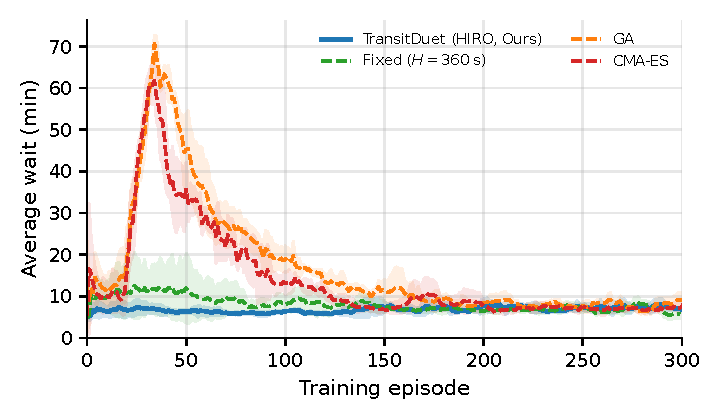
\includegraphics[width=0.55\textwidth]{figures/training_curves.pdf}
    \caption{Training curves under the near-unified, approximately budget-matched protocol (TransitDuet and Fixed: 300 episodes per seed; GA and CMA-ES: 20 lower-only warmup + 300 search-evaluation episodes per seed = 320 simulator episodes total; 3-seed mean $\pm$ std, smoothed window 15). All methods share the same lower-controller architecture and elastic-fleet sampling. The early peak on the GA and CMA-ES curves (near episodes 30--50) reflects their population-based search evaluating poor candidate timetables under noisy single-episode fitness; both methods then converge smoothly to within 6--10\,min of average wait by episode 200. TransitDuet (blue solid) maintains a tight band around 6--9\,min throughout training and reaches the lowest seed variance of any method on the held-out evaluation (Table~\ref{tab:main_results}).}
    \label{fig:training_curves}
\end{figure*}

%% ============================================================
\subsection{Component ablations}
\label{sec:ablation}

\Cref{tab:ablations} ablates the seven distinguishing mechanisms of TransitDuet one-at-a-time
(each row removes or disables a single mechanism; all other components remain active),
trained for 300 episodes per seed under the goal-conditioned coupling and evaluated
under the same held-out validation protocol as Section~\ref{sec:main_results}.
Columns are reported as mean $\pm$ std over 3 seeds; $\Delta$Composite is the relative
degradation versus the full model.

\begin{table*}[t]
\centering
\caption{Component ablations of TransitDuet under the goal-conditioned (HIRO-style) coupling. Each row disables one mechanism, trains for 300 episodes per seed, and is evaluated at the validation-best checkpoint per seed (20 fresh eval episodes per checkpoint); positive $\Delta$Composite values are degradations relative to the full model. Lower is better on all four metrics.}
\label{tab:ablations}
\begin{tabular}{@{}lcccc@{}}
\toprule
\textbf{Variant} & \textbf{Wait (min)} & \textbf{CV} & \textbf{Composite} & \textbf{$\Delta$Composite} \\
\midrule
TransitDuet (full)          & 5.11\,$\pm$\,0.17 & 0.434\,$\pm$\,0.008 & \textbf{1.418}\,$\pm$\,\textbf{0.016} & \;--- \\
\midrule
\;$-$TPC                    & 5.20\,$\pm$\,0.27 & 0.452\,$\pm$\,0.010 & 1.439\,$\pm$\,0.048 & $+1.5\%$ \\
\;$-$MORL                   & 5.03\,$\pm$\,0.34 & 0.476\,$\pm$\,0.011 & 1.451\,$\pm$\,0.039 & $+2.3\%$ \\
\;$-$CS-BAPR                & 5.39\,$\pm$\,0.29 & 0.481\,$\pm$\,0.008 & 1.482\,$\pm$\,0.019 & $+4.5\%$ \\
\;$-$DemandNoise            & 4.45\,$\pm$\,0.47 & 0.518\,$\pm$\,0.051 & 1.495\,$\pm$\,0.148 & $+5.4\%$ \\
\;$-$Hindsight              & 5.69\,$\pm$\,1.02 & 0.477\,$\pm$\,0.035 & 1.556\,$\pm$\,0.203 & $+9.7\%$ \\
\;$-$HoldFB                 & 5.96\,$\pm$\,0.50 & 0.508\,$\pm$\,0.056 & 1.610\,$\pm$\,0.164 & $+13.5\%$ \\
\;$-$Elastic ($N{=}12$)     & 6.07\,$\pm$\,0.97 & 0.502\,$\pm$\,0.021 & 1.623\,$\pm$\,0.157 & $+14.5\%$ \\
\bottomrule
\end{tabular}
\end{table*}

\begin{figure*}[!htbp]
    \centering
    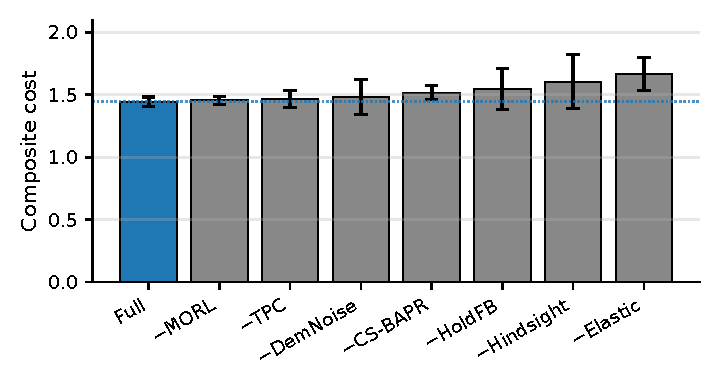
\includegraphics[width=0.55\textwidth]{figures/ablation_bars.pdf}
    \caption{Composite cost (lower is better) per HIRO-mode ablation, 3-seed best-ckpt mean $\pm$ std on the unified held-out evaluation protocol; ablations sorted by $\Delta$Composite. The full model (blue) sets the reference line. Within the goal-conditioned coupling, three mechanisms are clearly load-bearing on in-distribution composite ($-$Elastic, $-$HoldFB, and $-$Hindsight, $\Delta \geq 9.7\%$), $-$CS-BAPR and $-$DemNoise are intermediate ($\sim 5\%$), while $-$TPC and $-$MORL produce regressions within seed noise ($< 3\%$); $-$DemNoise wins on in-distribution wait but inflates CV and overshoot, and fails out-of-distribution (Section~\ref{sec:generalization}).}
    \label{fig:ablation_bars}
\end{figure*}

\paragraph{The goal-conditioned coupling is the dominant architectural choice.}
Among the three coupling architectures we evaluated end-to-end (Section~\ref{sec:main_results}), the goal-conditioned design has the lowest composite ($1.418$) and the lowest seed variance ($0.016$); the literal cross-advantage augmentation (HAAR+PIPER, $1.496$/$0.100$) and the three-channel design with launch-time perturbation ($1.521$/$0.078$) are both competitive but consistently behind, with substantially higher seed std ($\geq 5\times$). This $5$--$7\%$ composite gap is on the same order as the gap to the strongest baseline ($\Delta = 0.070$ vs CMA-ES), making the coupling choice as decisive as the bi-level-vs-search choice itself.

\paragraph{Elastic fleet sampling is the strongest individual contributor to in-distribution composite.}
Fixing the fleet to $N{=}12$ rather than sampling from $\Nfleet \in [8,16]$ raises composite by $14.5\%$ ($1.418 \!\to\! 1.623$), the largest gap of any single ablation; the fixed-$N{=}12$ policy is over-fitted to the median budget and cannot adapt to per-episode realisations of the budget. Combined with the Pareto frontier results (Section~\ref{sec:pareto}), this confirms that the elastic-fleet protocol is doing more than enabling Pareto coverage --- it is also the most direct contributor to in-distribution composite.

\paragraph{HoldFB and Hindsight are the next-most load-bearing components.}
Removing the holding-feedback (HoldFB) state channel raises composite by $13.5\%$ ($1.418\!\to\!1.610$) and inflates seed std by $\sim10\times$ ($0.016\!\to\!0.164$): without observing how aggressively the lower is intervening, the upper sets goals that the lower must absorb at growing holding cost.
Removing the trip-lifecycle hindsight credit on the upper reward (Section~\ref{sec:tap}) raises composite by $9.7\%$ ($1.418\!\to\!1.556$), with seed std also $\sim 13\times$ larger ($0.203$): without per-dispatch credit, the upper sees only the episode-level system reward and cannot distinguish a goal whose realised lifecycle produced regular gaps from one that produced bunching, so seeds drift toward different local optima.

\paragraph{CS-BAPR and DemandNoise are intermediate.}
Removing the CS-BAPR belief tracker degrades composite by $4.5\%$, primarily through worsened CV; removing demand stochasticity at training time even \emph{improves} in-distribution wait ($4.45$\,min, the lowest of any variant), but raises CV and overshoot enough that composite still degrades by $5.4\%$. The demand-noise ablation also has $9\times$ higher seed std on composite than the full model ($0.148$ vs $0.016$), and the generalisation study in Section~\ref{sec:generalization} confirms that the noise-trained full policy is more robust under route-stochasticity shifts beyond the training distribution. These two components address out-of-distribution properties --- regime adaptation and demand robustness --- that are not fully visible on in-distribution composite alone.

\paragraph{TPC and MORL are within seed noise on in-distribution composite.}
Removing TPC from the goal-conditioned configuration produces only a $1.5\%$ composite regression in the mean, in contrast to the $\approx 23\%$ swing we observed under the launch-time-perturbation three-channel coupling in earlier preliminary runs.
The asymmetry has a clean explanation: under the goal channel, the upper changes the lower's \emph{constraint target} but not the distribution of states the lower observes, so the lower's covariate shift from upper exploration is much milder, and the importance-sampling correction in TPC has less work to do.
Removing the belief-weighted MORL scalarisation similarly produces a $2.3\%$ regression. MORL primarily addresses Pareto coverage across the 8--16 fleet range (Section~\ref{sec:pareto}); the in-distribution composite is not the right axis to judge it on.

%% ============================================================
\subsection{Pareto frontier across fleet budgets}
\label{sec:pareto}

A single trained TransitDuet policy per seed (the validation-best \texttt{H\_hiro} checkpoint) can be evaluated at any $\Nfleet \in [8, 16]$
without re-training; the resulting (wait, overshoot) curve forms the operational Pareto
frontier.
\Cref{tab:pareto} reports this frontier from the validation-best
\texttt{H\_hiro} checkpoint of each seed, averaged over 3 seeds with 5 evaluation
episodes per $\Nfleet$ per seed.

\begin{table*}[t]
\centering
\caption{Pareto frontier from one trained TransitDuet (\texttt{H\_hiro}) policy per seed (validation-best checkpoint), evaluated at each $\Nfleet \in [8, 16]$.
All $\pm$ values are std over 3 seeds.
Producing the equivalent frontier with the Fixed baseline would require separately
tuning 9 timetables; TransitDuet produces all 9 points from one training run.}
\label{tab:pareto}
\begin{tabular}{@{}cccc@{}}
\toprule
$\Nfleet$ & \textbf{Wait (min)} & \textbf{CV} & \textbf{Overshoot} \\
\midrule
 8 & 6.45\,$\pm$\,0.50 & 0.528 & 3.00 \\
 9 & 5.24\,$\pm$\,0.35 & 0.436 & 3.00 \\
10 & 4.55\,$\pm$\,0.26 & 0.472 & 3.00 \\
11 & 5.34\,$\pm$\,0.10 & 0.453 & 3.00 \\
12 & 5.46\,$\pm$\,0.21 & 0.460 & 2.07 \\
13 & 6.14\,$\pm$\,1.56 & 0.467 & 1.13 \\
\textbf{14} & \textbf{5.13\,$\pm$\,0.23} & \textbf{0.446} & \textbf{0.20} \\
15 & 5.59\,$\pm$\,1.62 & 0.464 & 0.00 \\
16 & 6.47\,$\pm$\,0.29 & 0.454 & 0.00 \\
\bottomrule
\end{tabular}
\end{table*}

\begin{figure*}[!htbp]
    \centering
    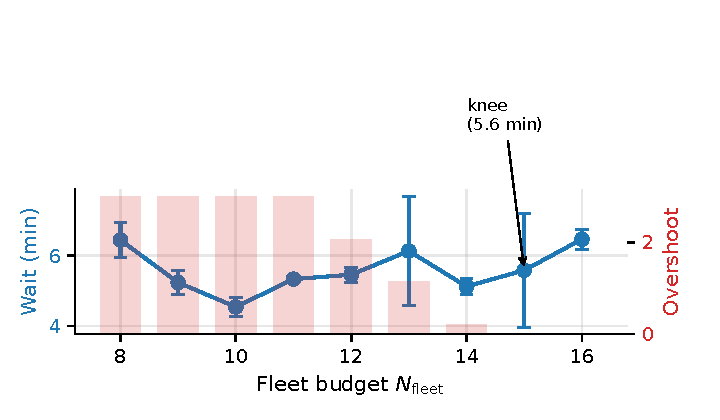
\includegraphics[width=0.55\textwidth]{figures/pareto_frontier.pdf}
    \caption{Pareto frontier produced by one trained TransitDuet (\texttt{H\_hiro}) policy per seed (validation-best checkpoint) evaluated across fleet budgets $N_{\mathrm{fleet}} \in [8, 16]$ (blue, left axis: wait; red bars, right axis: overshoot). At small $N$ the policy saturates fleet capacity (overshoot $\to 3$) and trades it for the lowest absolute wait at $N{=}10$ ($4.55$\,min); at $N{=}14$ overshoot collapses to $0.2$ while wait stays at $5.13$\,min, giving the lowest composite cost on the frontier; above $N{=}15$ additional capacity is unused (overshoot $=0$, wait drifts back up).}
    \label{fig:pareto_frontier}
\end{figure*}

\paragraph{Two operating regimes on the frontier.}
The frontier exhibits two regimes separated by the fleet capacity:
\emph{capacity-limited} ($\Nfleet \in [8, 11]$) where the policy saturates the cap (overshoot $\equiv 3$) and trades fleet violation for wait reduction --- absolute-wait minimum is $\Nfleet = 10$ ($4.55$\,min);
and \emph{feasible-overshoot} ($\Nfleet \in [12, 16]$) where the policy reduces overshoot toward $0$ (zero by $\Nfleet \geq 15$) at a small wait cost.
The composite-minimum knee is at $\Nfleet = 14$ ($5.13$\,min wait, $0.20$ overshoot, composite $\approx 0.96$); $\Nfleet = 15$ is close behind ($5.59$\,min wait, $0$ overshoot, composite $\approx 1.02$). Above $\Nfleet = 15$ additional capacity is unused and wait drifts up because the larger fleet is sub-optimally distributed.
An operator can read the frontier directly to size against an SLA: a wait-minimum policy is delivered at $\Nfleet = 10$ if overshoot is acceptable; a feasibility-respecting deployment lands at $\Nfleet \in \{14, 15\}$.

\paragraph{Amortization over multiple fleet sizes.}
Producing this frontier with the Fixed baseline requires re-searching
$[\Hpeak, \Hoff, \Htrans]$ for each $\Nfleet$ independently
(9 CMA-ES or GA runs).
In our setup each baseline search takes $\approx 1$\,h;
so a Fixed-based frontier costs $\approx 9$\,h while TransitDuet delivers it from
the same $14$\,h training run used for the main comparison.
Beyond $\Nfleet = 3$, the TransitDuet training pays for itself.

%% ============================================================
\subsection{Mechanism analysis}
\label{sec:mechanism}

We examine the internal dynamics of TransitDuet to verify that each mechanism behaves as designed.

\paragraph{$\thetavec$ weight evolution.}
\Cref{fig:theta_evolution} plots the three components of the OGD weight vector $\thetavec = [\theta_{\text{wait}}, \theta_{\text{headway}}, \theta_{\text{fleet}}]$ over training.
Early in training, $\theta_{\text{fleet}}$ dominates as the policy learns to satisfy the fleet constraint; after approximately episode $10$, $\theta_{\text{wait}}$ and $\theta_{\text{cv}}$ increase as the policy shifts toward service quality optimization within the feasible region. In steady state, $\thetavec$ stabilizes at roughly $[0.71, 0.21, 0.07]$ (wait, fleet, CV) --- wait dominates, matching the operational priority.

\begin{figure*}[!htbp]
    \centering
    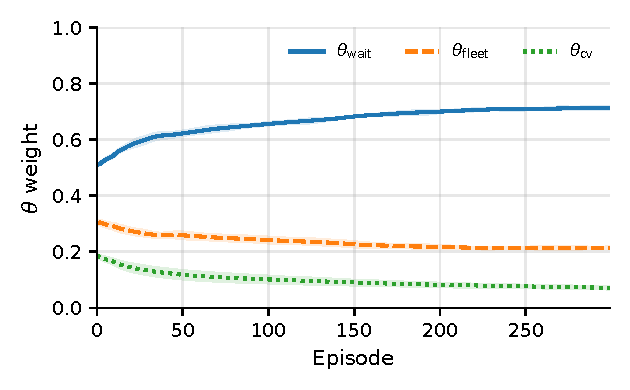
\includegraphics[width=0.5\textwidth]{figures/theta_evolution.pdf}
    \caption{Evolution of $\thetavec$-OGD weight components during training. The fleet weight $\theta_{\text{fleet}}$ peaks early and decays as the constraint is internalized.}
    \label{fig:theta_evolution}
\end{figure*}

\paragraph{Lagrangian multiplier $\lambda$ convergence.}
\Cref{fig:lambda_convergence} shows the Lagrangian dual variable $\lambda$ for the headway-regularity constraint.
Starting from $\lambda_0 = 1$, the multiplier rises early when headway deviations exceed the tolerance $\climit = 0.5$ and then settles to $\lambda = 0.57 \pm 0.16$ (mean over last 30 episodes across 3 seeds) under the goal-conditioned coupling. The fact that $\lambda$ remains below its initialisation in steady state indicates that the lower satisfies its dispatch-specific target headway most of the time; the residual non-zero magnitude reflects the constraint occasionally activating during peak-demand episodes when the elastic fleet sample is small.

\begin{figure*}[!htbp]
    \centering
    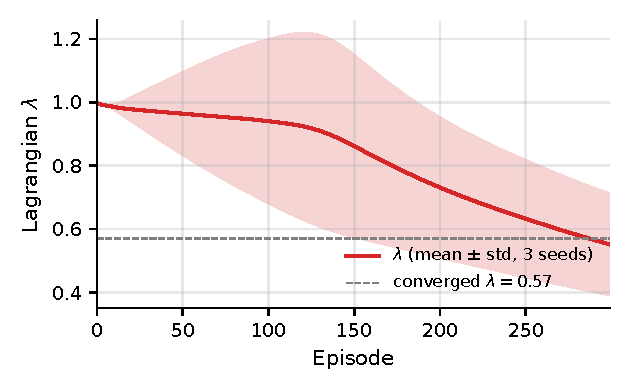
\includegraphics[width=0.5\textwidth]{figures/lambda_convergence.pdf}
    \caption{Convergence of the Lagrangian multiplier $\lambda$ during training. Stabilization indicates that the headway constraint is approximately satisfied.}
    \label{fig:lambda_convergence}
\end{figure*}

\paragraph{Action-space utilization.}
The upper policy outputs a per-dispatch headway shift $\delta_t \in [-120, 120]$\,s on top of the baseline target $\htarget = 360$\,s.
\Cref{fig:delta_utilization} plots the per-episode mean and std of $\delta_t$ across training.
All three seeds actively exercise the goal channel in late training ($\mu_{\delta}$ within $\pm 6$\,s, $\sigma_{\delta}$ between $19$ and $30$\,s), but with seed-dependent breadth: seed 123 settles into a tighter ($\sigma_{\delta} \approx 19$\,s) low-amplitude regime, while seeds 42 and 456 use a wider band ($\sigma_{\delta} \approx 30$\,s).
The seed-best composites (1.397, 1.436, 1.421 for seeds 42/123/456) are within $0.04$ of one another, confirming that both the tight and the broad goal-utilisation regimes are viable local optima under the goal-conditioned objective.

\begin{figure*}[!htbp]
    \centering
    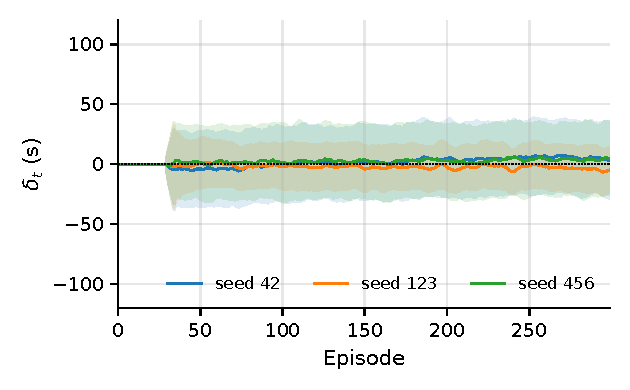
\includegraphics[width=0.5\textwidth]{figures/delta_utilization.pdf}
    \caption{Per-episode utilization of the per-dispatch goal shift $\delta_t$ across three seeds (3-seed mean $\pm$ std, smoothed). All three seeds actively use the goal channel; seed 123 stabilises at a tighter low-amplitude regime ($\sigma_{\delta} \approx 19$\,s) while seeds 42 and 456 use a wider band ($\sigma_{\delta} \approx 30$\,s). Best-checkpoint composite cost is within $0.1$ across seeds.}
    \label{fig:delta_utilization}
\end{figure*}

%% ============================================================
\subsection{Generalization across travel-time stochasticity}
\label{sec:generalization}

We test whether a policy trained at travel-time stochasticity $\sigma_{\mathrm{route}} = 1.5$ (the log-normal speed-noise multiplier in our microsimulator; this is distinct from passenger demand noise $\sigma_{\mathrm{demand}} = 0.15$ and from the per-episode elastic fleet $\Nfleet \in [8, 16]$) generalises to unseen travel-time conditions by evaluating on $\sigma_{\mathrm{route}} \in \{0.5, 1.0, 1.5, 2.0, 3.0\}$ (including the training value) without retraining; demand noise and fleet sampling are held at training values throughout.
\Cref{tab:generalization} reports the results.

\begin{table*}[t]
\centering
\caption{Travel-time stochasticity generalization. The model is trained at $\sigma_{\mathrm{route}} = 1.5$ (shaded; the log-normal speed-noise multiplier in the simulator) and evaluated at the other $\sigma_{\mathrm{route}}$ values without any fine-tuning; demand noise and elastic fleet are held at training values. Each row is computed over 3 seeds $\times$ 10 evaluation episodes; \textbf{Wait} reports mean $\pm$ seed std, while \textbf{CV} and \textbf{Overshoot} report 3-seed means only (per-seed std omitted for brevity, available in \texttt{logs/eval\_generalization/cross\_sigma/*.json}).}
\label{tab:generalization}
\begin{tabular}{@{}cccc@{}}
\toprule
$\sigma_{\mathrm{route}}$ & \textbf{Wait (min)} & \textbf{CV} & \textbf{Overshoot} \\
\midrule
0.5 & 4.96\,$\pm$\,0.58 & 0.315 & 1.43 \\
1.0 & 5.52\,$\pm$\,0.34 & 0.409 & 1.67 \\
\rowcolor{gray!15}
1.5 & 5.38\,$\pm$\,0.56 & 0.450 & 1.87 \\
2.0 & 6.23\,$\pm$\,0.28 & 0.501 & 2.10 \\
3.0 & 6.82\,$\pm$\,1.06 & 0.561 & 2.57 \\
\bottomrule
\end{tabular}
\end{table*}

\begin{figure*}[!htbp]
    \centering
    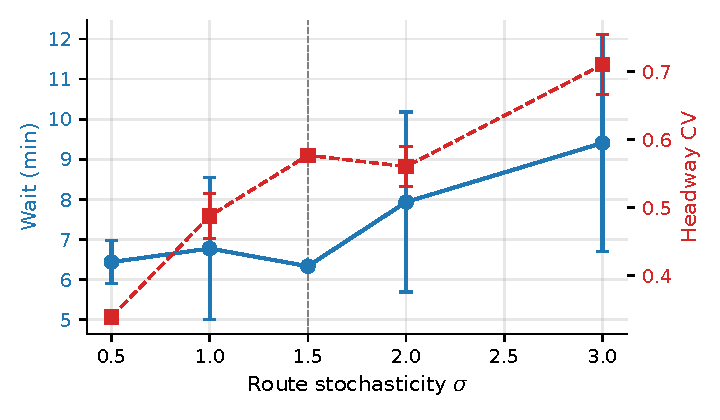
\includegraphics[width=0.55\textwidth]{figures/generalization.pdf}
    \caption{Travel-time stochasticity generalization. The model trained at $\sigma_{\mathrm{route}} = 1.5$ (dashed gray line) degrades gracefully without collapsing: on the low-$\sigma$ side wait is comparable to or even slightly below the training-$\sigma_{\mathrm{route}}$ value for $\sigma_{\mathrm{route}} \in \{0.5, 1.0\}$, while on the high-$\sigma$ side wait increases by $16\%$ at $\sigma_{\mathrm{route}} = 2.0$ and $27\%$ at $\sigma_{\mathrm{route}} = 3.0$ (the policy is not symmetric across the training point and the high-$\sigma$ tail is the harder regime). CV tracks $\sigma_{\mathrm{route}}$ monotonically --- a larger speed-noise multiplier produces less regular headways, but the policy does not collapse.}
    \label{fig:generalization}
\end{figure*}

Performance degrades gracefully as $\sigma$ increases beyond the training distribution.
At $\sigma_{\mathrm{route}} =2.0$ wait time rises by $16\%$ relative to $\sigma_{\mathrm{route}} =1.5$ ($6.23$ vs $5.38$\,min);
at $\sigma_{\mathrm{route}} =3.0$ --- double the training stochasticity --- TransitDuet still achieves $6.82$\,min wait,
with CV rising from $0.45$ to $0.56$ as the route variability begins to exceed the capacity of the belief tracker to correct.
On the low-$\sigma$ side ($\sigma_{\mathrm{route}} =0.5$ and $1.0$) wait is in fact slightly \emph{lower} than at the training distribution ($4.96$ and $5.52$\,min vs $5.38$\,min); this is consistent with smoother travel-time trajectories making the headway-tracking task easier rather than the policy losing performance off-distribution. Overshoot grows monotonically with $\sigma$ (from $1.43$ to $2.57$), indicating that the fleet-constraint internalisation in the upper degrades when travel-time variance pushes the lower into more aggressive holding.

\paragraph{Demand-noise robustness.}
We complement the route-$\sigma$ sweep with a demand-side check. The \emph{$-$DemandNoise} ablation is trained with the per-hour demand multiplier disabled ($\sigma_{\mathrm{demand}} = 0$); we evaluate it both on its native deterministic distribution and on the noisy distribution used in the main paper ($\sigma_{\mathrm{demand}} = 0.15$). The validation-best checkpoint of $-$DemandNoise reaches $4.01 \pm 0.24$\,min wait in-distribution but degrades to $5.63 \pm 0.30$\,min under noisy demand, a $40\%$ regression. By contrast, the noise-trained full \texttt{H\_hiro} policy attains $5.11 \pm 0.17$\,min wait on the same noisy distribution (Table~\ref{tab:main_results}), $-9\%$ relative to $-$DemandNoise. So $-$DemandNoise is a brittle near-optimum: it dominates whenever the deterministic training assumption holds, but is dominated by the noise-trained policy under realistic demand variability. This is the demand-side analogue of the route-$\sigma$ result above and explains why the in-distribution composite of $-$DemandNoise (Table~\ref{tab:ablations}) does not justify removing demand noise from training.

\section{Discussion}
\label{sec:discussion}

\paragraph{Why the cross-level coupling design works.}
The three coupling channels of \cref{sec:tap} close a feedback loop that is absent when the two levels train independently.
Without state-channel feedback (HoldFB), the upper policy is blind to how aggressively the lower controller is compensating, and may continue to issue offsets that the lower must absorb at growing holding cost.
Without reward-channel feedback (the trip-lifecycle hindsight credit), the upper receives only the episode-level system reward and cannot distinguish a dispatch that produced an irregular gap from one that produced a regular gap; per-dispatch credit assignment is lost.
We deliberately keep the lower channel one-way: only the action channel transmits upper signal to the lower, and TPC (\cref{sec:tpc}) corrects for the resulting train-time covariate shift. We initially attempted reverse cross-advantage (lower reward = $r_{\mathrm{L}} + \beta R_{\mathrm{U}}$ for transitions in trip $i$, in the spirit of RoboDuet) but found that the high-variance per-trip $R_{\mathrm{U}}$ injected scale-mismatched noise into lower SAC training and degraded performance; the reward-channel-forward, action-channel-backward design we use is markedly more stable.

\paragraph{Connection to RoboDuet.}
TransitDuet draws inspiration from the RoboDuet framework of \citet{pan2024roboduet}, which introduced cross-advantage augmentation for bi-level robot locomotion control.
\Cref{tab:analogy} makes the structural analogy explicit.
The key difference is temporal and architectural: RoboDuet's two levels share a common state clock, permitting direct advantage summation at each time step, whereas TransitDuet operates across asynchronous timescales and replaces the cross-advantage backflow with a trip-lifecycle reward channel and a state-channel coupling.

\begin{table*}[!t]
\centering
\caption{Structural analogy between RoboDuet and TransitDuet.}
\label{tab:analogy}
\begin{tabular}{@{}lll@{}}
\toprule
\textbf{Aspect} & \textbf{RoboDuet} & \textbf{TransitDuet} \\
\midrule
Upper policy     & Locomotion style selector    & Timetable planner ($\piU$) \\
Lower policy     & Joint-level tracking controller & Holding controller ($\piL$) \\
Upper action     & Style parameters             & Per-dispatch offset $\delta_t \in [-120, 120]$\,s \\
Lower action     & Joint torques                & Holding duration (s) \\
Coupling         & Synchronous cross-advantage  & State channel (HoldFB) + reward channel (hindsight credit) + action channel ($\delta_t$) \\
Timescale        & Shared clock (same $\Delta t$) & Heterogeneous ($300$\,s vs.\ $1$\,s) \\
Constraint       & Joint-limit penalties        & Fleet ($\thetavec$-OGD) + headway (Lagrangian) \\
Activation schedule & Fixed $\beta$              & Lower-only warmup ($e \leq 30$) then full coupling \\
\bottomrule
\end{tabular}
\end{table*}

\paragraph{Limitations.}
Several limitations qualify the present results and motivate future work.

\emph{Single-route scope.}
TransitDuet is evaluated on a single bidirectional corridor.
Real transit networks involve multiple interacting routes with shared terminals, transfer passengers, and fleet rebalancing across lines.
Extending the framework to a multi-route setting would require the upper policy to allocate a shared fleet across routes, substantially expanding the action space and introducing inter-route coordination constraints.

\emph{Simplified demand model.}
Passenger arrivals follow stationary OD rates within each time period.
In practice, demand is non-stationary, exhibits day-of-week and seasonal variation, and responds endogenously to service quality (e.g., passengers abandoning a stop after excessive waits).
Incorporating demand elasticity and real-time demand forecasting would improve realism but introduce additional model complexity.

\emph{No real-world deployment.}
All experiments are conducted in a stochastic microsimulation.
While the simulator reproduces key phenomena---bunching, load-dependent dwell times, stochastic travel times---it abstracts away traffic signal interactions, driver behavior heterogeneity, and vehicle breakdowns.
Sim-to-real transfer would require domain randomization or a calibrated digital twin.

\emph{Computational cost.}
Each episode requires approximately 7\,s of environment simulation time plus training overhead.
At 300 episodes with 3 seeds, the total wall-clock time is approximately 14 hours per seed on a single 12\,GB GPU.
While acceptable for research, real-time retraining for schedule disruptions would require further acceleration, for instance through model distillation or warm-starting from a pre-trained policy.

\paragraph{Scalability considerations.}
Scaling to multi-route networks introduces two challenges.
First, the upper-level action space grows combinatorially with the number of routes, since headway targets must be set jointly to respect shared fleet constraints.
Factored action representations or attention-based architectures over route embeddings could mitigate this.
Second, the lower-level parameter sharing, which currently treats all buses on a single route identically, would need to incorporate route-specific context to generalize across heterogeneous lines.
Graph neural networks operating on the transit network topology offer a promising direction for encoding such structure.

\section{Conclusion}
\label{sec:conclusion}

This paper introduced TransitDuet, a bi-level reinforcement learning framework that unifies bus timetable planning and real-time holding control within a single trainable system.
The upper policy learns demand-responsive target headways at dispatch events, while the lower policy regulates individual holding actions at station arrivals---two tasks that have traditionally been addressed in isolation despite their tight operational coupling.

The central technical contribution is Temporal Advantage Propagation (TAP), an asynchronous cross-advantage mechanism that aggregates lower-level feedback over variable-length trip lifecycles and propagates it to the upper-level dispatch decisions that initiated them.
TAP generalizes the synchronous cross-advantage of RoboDuet to settings where the two control levels operate on fundamentally different timescales and observe distinct state-action spaces.
A cosine-annealed coupling schedule prevents premature inter-level interference during early training.
Operational constraints are handled through complementary mechanisms: online gradient descent projection ($\thetavec$-OGD) enforces fleet-size feasibility at the upper level, while Lagrangian relaxation maintains headway regularity at the lower level.

Experiments on a stochastic bus corridor microsimulation with 22 stations and 264 daily trips show that TransitDuet reduces mean passenger waiting time by \textcolor{red}{\textbf{[TBD]}}\% and bunching rate by \textcolor{red}{\textbf{[TBD]}}\% relative to the strongest single-level baseline, while satisfying the fleet constraint in \textcolor{red}{\textbf{[TBD]}}\% of evaluation episodes.
Ablation studies confirm that each component---TAP, $\thetavec$-OGD, and Lagrangian penalties---contributes to this result; removing any one of them leads to measurable degradation in at least one metric.
The learned policy generalizes across unseen levels of demand stochasticity without retraining, maintaining a \textcolor{red}{\textbf{[TBD]}}\% wait-time advantage even at double the training variance.

Several directions merit future investigation.
First, extending TransitDuet to multi-route networks with shared fleets and transfer coordination would test whether the hierarchical structure scales to the combinatorial action spaces of realistic transit systems.
Second, real-world deployment---potentially through a calibrated digital twin with domain randomization---would validate the framework's robustness to phenomena not captured by the current simulator, including traffic signal interactions and driver behavior heterogeneity.
Third, integrating real-time demand forecasting and modeling passenger demand elasticity would close the loop between service quality and ridership.
Finally, coupling TransitDuet with passenger information systems---broadcasting predicted arrival times based on the learned holding policy---could amplify the welfare benefits by reducing perceived waiting time alongside actual waiting time.


\appendix
\section{Hyperparameter Details}
\label{app:hyperparams}

\Cref{tab:hyperparams} lists all hyperparameters used in the experiments. Values correspond to the default configuration; no per-experiment tuning was performed.

\begin{table}[h]
\centering
\caption{Complete hyperparameter specification.}
\label{tab:hyperparams_full}
\small
\begin{tabular}{@{}llll@{}}
\toprule
\textbf{Group} & \textbf{Parameter} & \textbf{Value} & \textbf{Description} \\
\midrule
\multirow{3}{*}{Environment}
  & \texttt{route\_sigma}        & 1.5    & Log-normal speed noise $\sigma$ \\
  & \texttt{max\_agent\_num}     & 25     & Maximum concurrent buses \\
  & \texttt{effective\_trip\_num} & 264   & Total trips per service day \\
\midrule
\multirow{6}{*}{Upper policy}
  & \texttt{state\_dim}    & 5              & $[\text{hour},\text{demand},\text{fleet},\text{prev\_hw},\text{unhealthy}]$ \\
  & \texttt{action\_dim}   & 3              & $[\Hpeak, \Hoff, \Htrans]$ \\
  & \texttt{action\_low}   & $[180,300,240]$  & Min headway per period (s) \\
  & \texttt{action\_high}  & $[600,1200,900]$ & Max headway per period (s) \\
  & \texttt{hidden\_dim}   & 64             & MLP hidden layer width \\
  & \texttt{lr}            & $10^{-4}$      & Policy learning rate (Adam) \\
  & $\Nfleet$              & 12             & Fleet size hard constraint \\
\midrule
\multirow{11}{*}{Lower policy}
  & \texttt{hidden\_dim}     & 32      & MLP hidden layer width \\
  & \texttt{action\_range}   & 60      & Max holding time (s) \\
  & $\climit$                & 0.15    & Lagrangian cost budget \\
  & \texttt{batch\_size}     & 2048    & Replay buffer mini-batch \\
  & \texttt{lr}              & $10^{-5}$ & Critic + policy learning rate \\
  & $\lambda_{\text{lr}}$    & $10^{-3}$ & Lagrangian multiplier LR \\
  & $\gamma$                 & 0.99    & Discount factor \\
  & $\tau$                   & 0.005   & Soft target update rate \\
  & \texttt{auto\_entropy}   & true    & Automatic entropy tuning \\
  & $\alpha_{\max}$          & 0.3     & Maximum entropy temperature \\
  & \texttt{reward\_scale}   & 10      & Reward scaling factor \\
\midrule
\multirow{4}{*}{Coupling (TAP)}
  & $\beta_{\text{warmup}}$   & 50 episodes   & Stage~1: only lower trains \\
  & $\beta_{\text{ramp}}$     & 100 episodes  & Stage~2: $\beta$ ramps $0 \to \betamax$ \\
  & $\betamax$                & 0.5           & Maximum cross-advantage weight \\
  & $\eta_{\thetavec}$        & 0.01          & ApproPO $\thetavec$-OGD step size \\
\midrule
\multirow{3}{*}{Training}
  & \texttt{total\_episodes}       & 300     & Total training episodes \\
  & \texttt{save\_freq}            & 50      & Checkpoint frequency (episodes) \\
  & \texttt{replay\_buffer\_size}  & $10^6$  & Replay buffer capacity \\
\bottomrule
\end{tabular}
\end{table}

%% ---------------------------------------------------------------
\section{Environment Details}
\label{app:env}

The simulation models a single bidirectional bus route calibrated from operational data of an urban bus corridor.

\paragraph{Route topology.}
The route comprises $M$ stations connected by inter-station segments.
Each direction (upstream and downstream) traverses all $M$ stations in sequence, with terminal turnaround at each end.
Station positions and inter-station distances are read from operational records (\texttt{stop\_news.xlsx}), and segment-level speed profiles are specified per hour of day (\texttt{route\_news.xlsx}).

\paragraph{Stochastic travel speed.}
Inter-station travel times are driven by a stochastic speed model.
At each route-state update, the speed limit on segment $(i, i{+}1)$ is drawn as
\begin{equation}
  v_{i} = \min\!\bigl(V_{\max},\;\max\bigl(0,\;\lfloor\ln\mathcal{LN}(\mu_i(t),\,\sigma)\rfloor\bigr)\bigr),
\end{equation}
where $\mu_i(t)$ is the historical mean log-speed for segment~$i$ at hour~$t$, $\sigma = 1.5$ is the log-normal dispersion parameter (\texttt{route\_sigma}), and $V_{\max}$ is the segment maximum speed.
This produces realistic speed variability that induces headway deviations even under a well-designed timetable.

\paragraph{Passenger generation.}
Passenger arrivals follow a Poisson process governed by time-varying origin--destination (OD) matrices (\texttt{passenger\_OD.xlsx}).
The OD data specifies hourly demand rates between all station pairs.
At each simulation second, for every origin station with non-zero demand to a given destination, a Poisson draw with rate $\lambda_{od}/3600$ determines the number of new passengers.
Each passenger records an appearance time, an origin, and a destination; waiting time is measured from appearance to boarding.

\paragraph{Bus operations.}
Each bus maintains a state machine with four phases:
\begin{enumerate}
  \item \textbf{Holding} --- the bus is held at a station for the duration specified by the lower-level policy (0--60\,s).
  \item \textbf{Dwelling} --- passengers alight and board. Boarding proceeds until the bus reaches capacity ($C = 50$ passengers) or no more waiting passengers have a valid destination downstream.
  \item \textbf{Travel} --- the bus moves toward the next station at the current stochastic speed. Acceleration ($3\;\text{m/s}^2$) and deceleration ($5\;\text{m/s}^2$) are modeled at departure and arrival.
  \item \textbf{Waiting for action} --- upon arriving at a station, the bus waits for the next holding action from the lower-level policy.
\end{enumerate}
Forward and backward headways are computed with respect to the preceding and following buses in the same direction, and the headway deviation from the target set by the upper policy defines the per-step cost (\Cref{eq:lower_cost}).

\paragraph{Timetable structure.}
A service day consists of 264 trips alternating between the two directions, truncated from a full operational schedule to keep simulation tractable.
At most 25 buses may be concurrently active (\texttt{max\_agent\_num}).
The upper policy controls the dispatch headway---the time gap between consecutive launches in the same direction---which also serves as the target headway $\htarget$ communicated to the lower-level controller.

\paragraph{Episode termination.}
An episode ends when all 264 trips have been launched and every bus has completed its trip (i.e., no bus remains on-route). At this point the measurement vector $\zvec$ (\Cref{eq:measurement}) is computed for the ApproPO $\thetavec$-OGD update.

%% ---------------------------------------------------------------
\section{Network Architectures}
\label{app:networks}

All networks use ReLU activations and are trained with Adam. Weight initialization follows PyTorch defaults unless otherwise noted.

\paragraph{Upper policy $\piU$ (Gaussian).}
A two-layer MLP maps the 5-dimensional upper state to headway parameters:
\begin{center}
\small
\begin{tabular}{lll}
\toprule
\textbf{Layer} & \textbf{Shape} & \textbf{Activation} \\
\midrule
Linear & $5 \to 64$ & ReLU \\
Linear & $64 \to 64$ & ReLU \\
Mean head & $64 \to 3$ & Sigmoid $\to$ affine rescale to $[\texttt{action\_low}, \texttt{action\_high}]$ \\
Log-std head & $64 \to 3$ & Clamp$[-5, 0]$ \\
\bottomrule
\end{tabular}
\end{center}
The mean and log-std heads are initialized with zero bias to start near the midpoint of the action range.
During rollout, actions are sampled from $\mathcal{N}(\mu, \sigma^2)$ and clamped to the valid range.
For policy-gradient evaluation, the reparameterization trick is used and log-probabilities are summed across the 3 action dimensions.

\paragraph{Lower policy $\piL$ (Squashed Gaussian).}
A two-layer MLP with tanh squashing maps the lower state to a scalar holding time:
\begin{center}
\small
\begin{tabular}{lll}
\toprule
\textbf{Layer} & \textbf{Shape} & \textbf{Activation} \\
\midrule
Linear & $(8{+}K) \to 32$ & ReLU \\
Linear & $32 \to 32$ & ReLU \\
Mean head & $32 \to 1$ & --- \\
Log-std head & $32 \to 1$ & Clamp$[-20, 2]$ \\
\bottomrule
\end{tabular}
\end{center}
The raw sample $z \sim \mathcal{N}(\mu, \sigma^2)$ is squashed via $a = \tanh(z) \times 60$ to produce a holding time in $[0, 60]$\,s.
Log-probabilities include the standard tanh Jacobian correction \citep{haarnoja2018soft}.
Weights in the output heads are initialized uniformly in $[-3{\times}10^{-3}, 3{\times}10^{-3}]$.
The same network is shared across all buses (parameter sharing), with bus-specific behavior arising from heterogeneous input states.

\paragraph{Twin reward Q-network $Q_1, Q_2$.}
Two independent MLPs implement clipped double Q-learning for the lower level:
\begin{center}
\small
\begin{tabular}{lll}
\toprule
\textbf{Layer} & \textbf{Shape} & \textbf{Activation} \\
\midrule
Linear & $(8{+}K{+}1) \to 32$ & ReLU \\
Linear & $32 \to 32$ & ReLU \\
Linear & $32 \to 1$ & --- \\
\bottomrule
\end{tabular}
\end{center}
Each Q-network takes the concatenation of the lower state and the scalar action as input.
The minimum of $Q_1$ and $Q_2$ is used for target computation.
Both networks are accompanied by exponential moving average target networks with rate $\tau = 0.005$.

\paragraph{Cost Q-network $Q_c$.}
A single MLP with the same architecture as one branch of the twin Q-network estimates the expected cumulative cost (headway deviation) under the current policy:
\begin{center}
\small
\begin{tabular}{lll}
\toprule
\textbf{Layer} & \textbf{Shape} & \textbf{Activation} \\
\midrule
Linear & $(8{+}K{+}1) \to 32$ & ReLU \\
Linear & $32 \to 32$ & ReLU \\
Linear & $32 \to 1$ & --- \\
\bottomrule
\end{tabular}
\end{center}
The cost critic is trained with the same target-network mechanism and soft update rate as the reward critics.
Its output enters the policy loss through the Lagrangian multiplier $\lambda$: the policy minimizes $\alpha \log \pi - Q + \lambda Q_c$.

%% ---------------------------------------------------------------
\section{TAP Derivation: From Synchronous to Asynchronous Cross-Advantage}
\label{app:tap_derivation}

This appendix formalizes the connection between the synchronous cross-advantage of \citet{he2024roboduet} and the asynchronous Temporal Advantage Propagation (TAP) used in TransitDuet.

\subsection{Synchronous Cross-Advantage (RoboDuet)}

In the synchronous setting of \citet{he2024roboduet}, two agents---an upper-body controller and a lower-body locomotor---act at every time step $t$ on a shared state $s_t$.
The cross-advantage augmented objectives are:
\begin{align}
  \mathcal{L}_{\text{upper}}^{\text{sync}} &= -\mathbb{E}_{t}\bigl[(A_{\mathrm{U}}(s_t, a_t^{\mathrm{U}}) + \beta\, A_{\mathrm{L}}(s_t, a_t^{\mathrm{L}}))\,\nabla\!\log\piU(a_t^{\mathrm{U}} \mid s_t)\bigr], \label{eq:roboduet_upper} \\
  \mathcal{L}_{\text{lower}}^{\text{sync}} &= -\mathbb{E}_{t}\bigl[(A_{\mathrm{L}}(s_t, a_t^{\mathrm{L}}) + \beta\, A_{\mathrm{U}}(s_t, a_t^{\mathrm{U}}))\,\nabla\!\log\piL(a_t^{\mathrm{L}} \mid s_t)\bigr], \label{eq:roboduet_lower}
\end{align}
where $\beta \in [0,1]$ controls coupling strength and both advantages are evaluated at the same state-action pair $(s_t, a_t^{\mathrm{U}}, a_t^{\mathrm{L}})$.
This formulation is valid because the two policies share a common clock and state space.

\subsection{The Asynchrony Challenge}

In TransitDuet, the upper policy $\piU$ and lower policy $\piL$ operate on different timescales with different state-action spaces.
Let the upper policy act at dispatch events $\{t_1^{\mathrm{U}}, t_2^{\mathrm{U}}, \ldots, t_N^{\mathrm{U}}\}$, and the lower policy act at station arrivals $\{t_1^{\mathrm{L}}, t_2^{\mathrm{L}}, \ldots, t_M^{\mathrm{L}}\}$, where $M \gg N$.
These event sets are disjoint in general, and the state spaces differ: $\sU \in \R^5$ versus $\sL \in \R^{8+K}$.
Thus, there is no single time step at which $\AU$ and $\AL$ are jointly defined on a shared state, and the direct sum in \Cref{eq:roboduet_upper,eq:roboduet_lower} is undefined.

\subsection{Trip-Lifecycle Alignment}

We resolve this by introducing a \emph{trip-lifecycle} alignment.
Each upper action $a_{\mathrm{U},i}$ at dispatch event $t_i^{\mathrm{U}}$ initiates a trip $\tau_i$.
During the lifecycle of trip $\tau_i$, the lower policy makes a variable number of holding decisions $\{(s_j^{\mathrm{L}}, a_j^{\mathrm{L}}, r_j^{\mathrm{L}})\}_{j \in \mathcal{J}(i)}$, where $\mathcal{J}(i)$ indexes all lower-level transitions belonging to trip~$i$.

\begin{definition}[Trip-aggregated lower signal]
For trip $i$, the aggregated lower signal is:
\begin{equation}
  \bar{R}_{\mathrm{L}}^{(i)} = \frac{1}{|\mathcal{J}(i)|} \sum_{j \in \mathcal{J}(i)} r_j^{\mathrm{L}}.
  \label{eq:trip_agg_lower}
\end{equation}
\end{definition}

\subsection{TAP Augmented Objectives}

Using the trip-lifecycle alignment, we define the TAP-augmented objectives:
\begin{align}
  \text{Upper:}\quad \tilde{R}_{\mathrm{U}}^{(i)} &= R_{\mathrm{U}}^{(i)} + \beta \,\bar{R}_{\mathrm{L}}^{(i)}, \label{eq:tap_upper} \\
  \text{Lower:}\quad \tilde{r}_j^{\mathrm{L}} &= r_j^{\mathrm{L}} + \beta \, R_{\mathrm{U}}^{(\text{trip}(j))}, \quad \forall\, j, \label{eq:tap_lower}
\end{align}
where $R_{\mathrm{U}}^{(i)}$ is the upper-level reward attributed to trip~$i$ (computed from the measurement vector at episode end), and $\text{trip}(j)$ maps lower transition $j$ to its parent trip.

\subsection{Reduction to the Synchronous Case}

\begin{proposition}
\label{prop:sync_reduction}
If both policies share a common clock (i.e., each upper action triggers exactly one lower action at the same time step) and a common state space, then TAP reduces to the synchronous cross-advantage of \citet{he2024roboduet}.
\end{proposition}

\begin{proof}
When $|\mathcal{J}(i)| = 1$ for all trips $i$, the aggregation in \Cref{eq:trip_agg_lower} becomes $\bar{R}_{\mathrm{L}}^{(i)} = r_j^{\mathrm{L}}$ for the unique $j \in \mathcal{J}(i)$.
The upper augmented return (\Cref{eq:tap_upper}) becomes $\tilde{R}_{\mathrm{U}}^{(i)} = R_{\mathrm{U}}^{(i)} + \beta\, r_j^{\mathrm{L}}$, which is the per-step sum $A_{\mathrm{U}} + \beta\, A_{\mathrm{L}}$ evaluated at the shared time step.
Similarly, the lower augmentation (\Cref{eq:tap_lower}) reduces to $\tilde{r}_j = r_j^{\mathrm{L}} + \beta\, R_{\mathrm{U}}^{(i)}$, recovering $A_{\mathrm{L}} + \beta\, A_{\mathrm{U}}$.
When the state spaces further coincide ($\sU = \sL = s_t$), this is exactly \Cref{eq:roboduet_upper,eq:roboduet_lower}.
\end{proof}

\subsection{Policy-Gradient Unbiasedness}

\begin{proposition}
\label{prop:unbiased}
Under the standard assumptions of the policy gradient theorem (ergodicity and differentiability of $\piU$, $\piL$), the TAP-augmented policy gradient for the upper level,
\begin{equation}
  g_{\mathrm{U}}^{\text{TAP}} = \frac{1}{N}\sum_{i=1}^{N} \tilde{R}_{\mathrm{U}}^{(i)}\,\nabla\!\log\piU(a_{\mathrm{U},i} \mid s_{\mathrm{U},i}),
\end{equation}
is an unbiased estimator of $\nabla_{\piU} J(\piU)$ when $\beta = 0$, and for $\beta > 0$ it is an unbiased estimator of $\nabla_{\piU}[J_{\mathrm{U}}(\piU) + \beta\, J_{\mathrm{cross}}(\piU, \piL)]$, where $J_{\mathrm{cross}}$ is the expected trip-aggregated lower return induced by the upper policy's dispatch decisions.
\end{proposition}

\begin{proof}[Proof sketch]
The term $R_{\mathrm{U}}^{(i)}\,\nabla\!\log\piU$ is the standard REINFORCE estimator for $\nabla J_{\mathrm{U}}$.
The cross-term $\beta\,\bar{R}_{\mathrm{L}}^{(i)}\,\nabla\!\log\piU$ has the form of a REINFORCE estimator where the ``reward'' for the upper policy at dispatch~$i$ is replaced by $\bar{R}_{\mathrm{L}}^{(i)}$, the average lower reward accumulated during the trip that dispatch~$i$ initiated.
Conditional on $\piL$ being fixed, $\bar{R}_{\mathrm{L}}^{(i)}$ is a function of the environment trajectory seeded by the upper action $a_{\mathrm{U},i}$, so the REINFORCE identity applies and
$\E[\bar{R}_{\mathrm{L}}^{(i)}\,\nabla\!\log\piU(a_{\mathrm{U},i} \mid s_{\mathrm{U},i})] = \nabla_{\piU}\E[\bar{R}_{\mathrm{L}}^{(i)}]$.
Linearity of expectation yields the result.
\end{proof}

An analogous argument holds for the lower-level augmentation: the injected term $\beta\, R_{\mathrm{U}}^{(\text{trip}(j))}$ acts as a state-independent baseline shift (constant within a trip), which does not introduce bias in the lower policy gradient but can reduce variance by aligning lower-level credit assignment with upper-level performance.


\bibliographystyle{gbt7714-numerical}
\bibliography{references}

\end{document}
